\documentclass[oneside,12pt,a4paper,openright]{report}
\usepackage{graphicx}
\usepackage{caption}
\usepackage{subcaption}
\usepackage{amsmath, amssymb, graphics, setspace, bbm}
\usepackage{listings}
\usepackage{color}
\usepackage{verbatim}
\usepackage{float}
\usepackage{xstring}
\usepackage{titletoc}
\usepackage{datetime}
\usepackage{layout}
\usepackage[utf8]{inputenc} % usually not needed (loaded by default)
\usepackage[T1]{fontenc}
\usepackage[nottoc]{tocbibind}
\usepackage{csquotes}
\usepackage{dsfont}
\usepackage{bbm}
\usepackage{epsfig}
\usepackage{physics}
\usepackage{enumitem}
\usepackage{hyperref}
\usepackage{textcomp}
\usepackage{hyperref}
\usepackage{geometry}
\usepackage{fancyhdr}
\usepackage{pdfpages}
\usepackage{xparse}
\usepackage{indentfirst}
\pdfminorversion=5
\usepackage{epstopdf}
\epstopdfDeclareGraphicsRule{.eps}{pdf}{.pdf}{%
  repstopdf --gsopt=-dCompatibilityLevel=1.5 #1 \OutputFile}
%\usepackage[style=apa]{biblatex}
\maxdeadcycles=200
%%%%%%%%%%%%%%%%%%%%%%%%%%%%%%%%%%%%%%%%%%%%%%%%%%%%%
% Enter the date that You want on the cover here:   %
%%%%%%%%%%%%%%%%%%%%%%%%%%%%%%%%%%%%%%%%%%%%%%%%%%%%%
\newdate{date}{03}{10}{2021}

%\setcounter{secnumdepth}{3}
%\setcounter{tocdepth}{3}

\newcommand{\HRule}{\rule{\linewidth}{0.5mm}}

%\setlength{\hoffset}{0pt}
%\setlength{\evensidemargin}{28pt}
%\setlength{\oddsidemargin}{79pt}
%\setlength{\textwidth}{345pt}
%\setlength{\marginparwidth}{15pt}
%\setlength{\hoffset}{0pt}
%\setlength{\evensidemargin}{28pt}
%\setlength{\oddsidemargin}{3.5cm}
%%\setlength{\textwidth}{345pt}
%\setlength{\marginparwidth}{1.6cm}
\linespread{1.0}
\usepackage{geometry}
 \geometry{
 a4paper,
 total={170mm,257mm},
 left=35mm,
 right=16mm,
 top=25mm,
 bottom=25mm
 }

 % links parameters
 \hypersetup{
    colorlinks=true,
    linkcolor=blue,
    urlcolor=red,
    pdftitle={Thesis Urbanevych},
    }

  % acronyms
 \usepackage[acronym, automake]{glossaries-extra}
\setabbreviationstyle[acronym]{long-short}

\newacronym{qcd}{QCD}{Quantum chromodynamics}
\newacronym{ceft}{$\chi$EFT}{Chiral effective field theory}
\newacronym{eft}{EFT}{effective field theory}
\makeglossaries


% chapter name
\usepackage[Conny]{fncychap}
%Options: Sonny, Lenny, Glenn, Conny, Rejne, Bjarne, Bjornstrup

\begin{document}

\newpage

%%%%%%%%%%%%%%%%%%%%%%%%%%%%%%%%%%%%%%%%%%%%%%%%%%%%%
% The titlepage starts here.                        %
%%%%%%%%%%%%%%%%%%%%%%%%%%%%%%%%%%%%%%%%%%%%%%%%%%%%%
\begin{titlepage}
\begin{center}

~\\[5cm]

%%%%%%%%%%%%%%%%%%%%%%%%%%%%%%%%%%%%%%%%%%%%%%%%%%%%%
% Enter Your title here:                            %
%%%%%%%%%%%%%%%%%%%%%%%%%%%%%%%%%%%%%%%%%%%%%%%%%%%%%
\HRule \\[0.4cm]
{ 
\huge \bfseries 
Application of the chiral forces to elctroweak processes
\\[0.4cm] 
}
\HRule \\[0.4cm]
%%%%%%%%%%%%%%%%%%%%%%%%%%%%%%%%%%%%%%%%%%%%%%%%%%%%%
% Enter Your name below:                            %
%%%%%%%%%%%%%%%%%%%%%%%%%%%%%%%%%%%%%%%%%%%%%%%%%%%%%
{
\LARGE
\bfseries
Vitalii Urbanevych
}
\vfill

%%%%%%%%%%%%%%%%%%%%%%%%%%%%%%%%%%%%%%%%%%%%%%%%%%%%%
% Enter details below:                              %
%%%%%%%%%%%%%%%%%%%%%%%%%%%%%%%%%%%%%%%%%%%%%%%%%%%%%
{
\large
Ph.D. thesis written under the supervision of dr. hab Roman Skibi\'nski \newline at the Jagiellonian University,
Faculty of Physics, Astronomy \newline and Applied Computer Science, Krak\'ow,
}
\\
{
\large \displaydate{date}
}
%\let\origdoublepage\cleardoublepage
%\newcommand{\clearemptydoublepage}{%
%  \clearpage
%  {\pagestyle{empty}\origdoublepage}%
%}

\end{center}
\begin{center}
	
\includegraphics[height = 0.1 \textheight]{her_pds_c.pdf}
\end{center}
\end{titlepage}

%%%%%%%%%%%%%%%%%%%%%%%%%%%%%%%%%%%%%%%%%%%%%%%%%%%%%
% This generates the table of contents.             %
%%%%%%%%%%%%%%%%%%%%%%%%%%%%%%%%%%%%%%%%%%%%%%%%%%%%%
\tableofcontents

%%%%%%%%%%%%%%%%%%%%%%%%%%%%%%%%%%%%%%%%%%%%%%%%%%%%%
% Import the abstract.                              %
%%%%%%%%%%%%%%%%%%%%%%%%%%%%%%%%%%%%%%%%%%%%%%%%%%%%%
%\begin{abstract}

%%%%%%%%%%%%%%%%%%%%%%%%%%%%%%%%%%%%%%%%%%%%%%%%%%%%%
% Enter jaw droping abstract below:                 % 
%%%%%%%%%%%%%%%%%%%%%%%%%%%%%%%%%%%%%%%%%%%%%%%%%%%%%

This Ph.D. thesis presents a comprehensive investigation into the application of the chiral potential to understand two types of processes with two- and three-nucleons. The primary focus is on the application of 
the state-of-the-art \gls{sms} potential to photodisintegration processes of $^2$H, $^3$H, and $^3$He,
as well as to pion absorption by the same nuclei.
The \gls{sms} potential is taken up to the fifth order of chiral expansion, N$^4$LO+, and augmented by the consistently regularized three-nucleon force at N$^2$LO.

The study employs the momentum space formalism, solving the standard Lippmann-Schwinger equation to obtain the $t$-operator and the corresponding two-nucleon scattering state. For three-nucleon processes, the Faddeev equations are utilized to include both initial and final state interactions, allowing a thorough examination of observables such as total cross sections, capture rates, differential cross sections, and polarization observables.

The main goal is to assess the quality and convergence of predictions based on the chiral \gls{sms} potential, particularly in comparison to the semi-phenomenological AV18 potential. The research explores the convergence of predictions with respect to the chiral order, revealing that predictions based on the \gls{sms} interaction are generally well-converged, indicating satisfactory model performance. Additionally, in this work I study the dependence of predictions on the intrinsic cut-off parameter $\Lambda$, providing valuable insights into the sensitivity of results to this parameter.

Furthermore, the study investigates the role of various dynamical components, including final state interactions and two-nucleon current contributions. The analysis highlights the significance of these components in influencing predicted values, emphasizing the importance of a fully consistent model incorporating 2N forces, 3N forces, and one-, two-, and three-body currents.

In conclusion, this work contributes to our understanding of electromagnetic and strong processes in nuclear physics, demonstrating the high quality and convergence of the chiral \gls{sms} potential.
For all studied processes I point out especially interesting observables and kinematical configurations, in which the role of individual components of the Hamiltonian is highlighted.
% The findings provide valuable insights for future developments in theoretical frameworks and emphasize the importance of comprehensive models for accurate predictions in nuclear physics.

This work is organized as follows. Chapter 1 provides an introduction to the theoretical framework and the motivation for the study. Chapter 2 presents the formalism and methodology used in the study. Chapter 3 presents the results of numerical calculations for corresponding processes, and Chapter 4 provides a summary and conclusions.

\tmp{zrobic rozrzerzoną wersję dla rady.}

\end{abstract}


%%%%%%%%%%%%%%%%%%%%%%%%%%%%%%%%%%%%%%%%%%%%%%%%%%%%%
% Input the chapters of the thesis.                 %
% The template has only two.                        %
%%%%%%%%%%%%%%%%%%%%%%%%%%%%%%%%%%%%%%%%%%%%%%%%%%%%%
%% \documentclass[twoside,12pt,a4paper]{report}
\linespread{1.15}
\usepackage{graphicx}
\usepackage{pgf}
\usepackage{fancyhdr}
\usepackage{dcolumn}
\usepackage{multirow}
\usepackage{amssymb}
\usepackage{amsbsy}
\usepackage{amsmath}
\usepackage{epsfig}
% \usepackage{epsfig,subfigure}
\usepackage{color}
\usepackage{bm}
\usepackage{verbatim} % needed for multi-line comments
\usepackage{rotating} % needed for sidewaystable
\usepackage{hhline}
\usepackage{xspace}
% \usepackage{subfigure}
\usepackage{anysize}
\usepackage{fixmath}
\usepackage{color}
\usepackage{cite}
\usepackage[toc,page]{appendix}
\usepackage[utf8]{inputenc}
\usepackage[T1]{fontenc}
\usepackage{comment}
\usepackage[acronym]{glossaries}
\usepackage{lineno} % package for line numebers, useful in review
\usepackage{titlesec}
\usepackage{titlesec}
\usepackage{braket}

\titleclass{\subsubsubsection}{straight}[\subsection]

\newcounter{subsubsubsection}[subsubsection]
\renewcommand\thesubsubsubsection{\thesubsubsection.\arabic{subsubsubsection}}

\titleformat{\subsubsubsection}
{\normalfont\normalsize\bfseries}{\thesubsubsubsection}{1em}{}
\titlespacing*{\subsubsubsection}{0pt}{3.25ex plus 1ex minus .2ex}{1.5ex plus .2ex}

\makeatletter
\renewcommand\paragraph{\@startsection{paragraph}{5}{\z@}%
	{3.25ex \@plus1ex \@minus.2ex}%
	{-1em}%
	{\normalfont\normalsize\bfseries}}
\renewcommand\subparagraph{\@startsection{subparagraph}{6}{\parindent}%
	{3.25ex \@plus1ex \@minus .2ex}%
	{-1em}%
	{\normalfont\normalsize\bfseries}}
\def\toclevel@subsubsubsection{4}
\def\toclevel@paragraph{5}
\def\toclevel@paragraph{6}
\def\l@subsubsubsection{\@dottedtocline{4}{7em}{4em}}
\def\l@paragraph{\@dottedtocline{5}{10em}{5em}}
\def\l@subparagraph{\@dottedtocline{6}{14em}{6em}}
\makeatother

\setcounter{secnumdepth}{4}
\setcounter{tocdepth}{4}


% \chapter*{Overview of the thesis}%Overview of thesis
\addcontentsline{toc}{chapter}{Overview of the thesis}
\label{overview}
One of the main goals of theoretical low-energy nuclear physics is to establish 
the structure of the nuclear Hamiltonian. Up to now, a large set of experimental data has 
been accumulated, both from elastic and inelastic nucleons scattering on nuclei 
over a wide range of energy. This is especially true for the elastic nucleon-deuteron 
(Nd) scattering and the nucleon-induced deuteron breakup processes. During many years of theoretical 
investigations of three-nucleon (3N) systems conducted among others, by the 
Krak{\' o}w-Bochum group, it was proved that 
using nucleon-nucleon (NN) force is not sufficient to provide an
accurate description of such systems. An additional 3N force (3NF)
is required to obtain a precise 
description of the 3N data~\cite{Witaa2001}. 
Nowadays, unfortunately, 
the details of 3N force are still poorly known and many efforts are undertaken to establish 
their properties. One example are calculations performed in the 
Krak{\'{o}}w-Bochum group that enabled experimentalists to prepare measurements 
sensitive to specific features of the nuclear Hamiltonians, the role of 
particular NN force components, charge independence breaking, and the structure of 
the 3NF. Major important results obtained before the mid-1990s for the 3N 
system were summarized in a review paper~\cite{Glockle1996}, which is an important 
reference for a reader interested in 3N calculations. 
%~\footnote{The deuteron is a bound state formed by a neutron and a proton 
%and is the only bound state of the two-nucleon (2N) system.} 
%this additional potential is different from a NN
%force in that it can not be written as a sum of pairwise interactions.
%Three nucleon systems are important because they allow the probing of
%the off-energy-shell properties of the 
%nuclear potential to study properties of 3N forces needed 

Moreover, in order to obtain reliable and accurate information from comparing 3N data with rigorous theoretical calculations it is necessary to estimate the uncertainties of theoretical predictions, in addition to the uncertainties of 3N data. Such estimation should start already when working with two-nucleon forces only. This would allow to estimate a contribution of 3NF in the description of various phenomena of nuclear physics. Of course such estimations should be confirmed by calculations which explicitly take into account NN interactions combined with 3NFs. 

In the past, for various reasons, the uncertainty budget for theory calculations in nuclear physics was not available or the estimated uncertainties did not offer a statistical interpretation.
With the increasing accuracy of experimental data in all areas of physics, for example in the three-nucleon sector, see, e.g., Refs.~\cite{Howell1994, Kistryn2005, Przewoski2006, Weisel2014, Sekiguchi2017}, 
the question of the uncertainty of theoretical predictions has became very relevant in the last decade.
For instance, the problem of uncertainty quantification of theoretical calculations was emphasized in an editorial in Physical Review A~\cite{edit2011} journal which covers atomic, molecular, and optical physics. 
This guideline was also taken by the nuclear physicist community.  
%A discussion of the importance of estimating uncertainties theoretical calculations was 
%recognized as one of the goals of theoretical low-energy nuclear physics, and 
%this guideline began to apply to nuclear physics theoretical calculations. 
As a result of intensive discussion, among others, the ISNET workshops (Information and Statistics in Nuclear Experiment and 
Theory) are organized in order to discuss issues related to the application of applied 
mathematics, information theory and statistics in the analysis of experiments,
and possibilities of calculating the uncertainties of relavent theoretical 
calculations. The 
first workshop resulted in a special issue of the \textit{Journal of Physics G: 
Nuclear and Particle Physics} (2015). Additionally, in the near future, the next \textit{J Phys G} 
special issue devoted to this subject will be published. In my studies I would like to contribute to these efforts and an important part of my thesis is devoted to studying some specific theoretical uncertainties.

For a specific case of elastic Nd scattering, the \textit{ab~initio} theoretical studies of 3N observables are possible 
using modern models of nuclear forces. NN force models used in such investigations contain a number 
of free parameters whose values are fixed from the 2N data. 
For my studies, the most important examples of such models are the new generation of the chiral 
interaction derived even beyond to the fifth-order (N$^{4}$LO) of the chiral expansion using the semilocal regularization 
in momentum space (SMS) by the Bochum-Bonn group~\cite{Reinert2018} and the semi-phenomenological 
One-Pion-Exchange-Gaussian (OPE-Gaussian) potential, proposed by the Granada group~\cite{NavarroPerez2014}. 
This choice is dictated by the availability of the covariance matrix for free parameters of these forces. 
The knowledge of the covariance matrix of the potential parameters opens new opportunities in studies of 
few-nucleon systems. 
One of them, realized in this thesis, is to determine the magnitude of uncertainty of the investigated observables (a so-called theoretical statistical error)
that arises from the propagation of uncertainty of NN potential parameters. Part of the results presented in the thesis has been shown 
in~\cite{Skibinski2018, volkotrub2020uncertainty}.
Another possibility is to investigate correlations among various 2N and 3N observables 
as well as between observables and specific potential parameters. The information 
about correlations among such observables is particularly interesting in the 
context of determining free strength parameters present in the 3N 
interaction. The values of these parameters are traditionally obtained by 
fixing from 3N data. However, using correlated 3N 
observables in such an analysis may lead to an inaccurate determination of the sought parameters. 
In this thesis I determine the correlations among 
3N observables in a statistically correct way, based on the relatively big 
sample of predictions. 

Summarizing, the main goal of this doctoral dissertation is the theoretical study of 3N observables for 
elastic and inelastic Nd scattering by using the newest semilocal momentum-space regularized 
chiral force. The first part of this work deals with various types of theoretical uncertainties of the 3N scattering observables. The statistical uncertainties obtained with the OPE-Gaussian potential and the chiral SMS interaction at different orders of chiral expansion are in the heart of my work. In addition to the $nd$ elastic scattering, the statistical uncertainties are compared with the truncation errors arising from the restriction to a specific order of chiral predictions, which can be done in two ways using a prescription suggested in~\cite{binder2016few, binder2018few} or within the Bayesian method~\cite{melendez2017bayesian}, and with the cutoff dependence of chiral predictions.
The second part of my thesis is devoted to collecting information about the correlations among all 2N and 3N elastic scattering observables as well as between observables and specific potential parameters. The knowledge, if some observables are or are not correlated, can impact future methods of fixing free parameters of the two- and many-body potentials. Especially the case of correlations in a 3N system should deliver information on possible restrictions on data sets used during fitting the 3NF parameters. In the case of correlations between potential parameters and 2N observables, the problem at hand is existence of observables that show strong sensitivity to a given part of the potential. If this is a case such an observable could be possibly used to fix this particular parameter. This, in turn, will reduce the number of remaining free parameters, which would simplify the rest of fitting procedure.

In the next Chapter I give a more elaborate introduction to my studies while in Chapter~\ref{potentials} I describe the two-nucleon force models which are used in investigations. In Chapter~\ref{application_cov_mat} I describe various types of theoretical uncertainties and usefulness of covariance matrix of two-nucleon potential parameters. In Chapter~\ref{formalism} I show the essential elements of our methods in computing the deuteron binding energy and 2N scattering observable, and the framework of the 3N Faddeev equations in computing 3N scattering observables used in my research. Chapter~\ref{error} is devoted to results for elastic scattering and breakup reactions. In Chapter~\ref{correlations} I show investigated correlations among various two- and three-nucleon observables as well as between observables and specific potential parameters. I summarize in Chapter.
%My work is also aimed at establishing the uncertainty quantification (UQ) of these observables. The part of my thesis is devoted to studying correlations among various few-nucleon scattering observables and between observables and potential parameters of NN forces.


%The manuscript is organized as follows. Chapter~\ref{introduction} gives a 
%brief overview of low-energy nuclear physics. In Chapter of this dissertation % TODO
%we show the essential elements of our formalism, describe briefly its numerical % TODO
%realization Equations for the 2N and 3N bound states % TODO
%%NN forces, which very accurately described the properties of the two-nucleon 
%(2N) system % TODO
%%
%%the nonrelativistic framework for the calculation of nucleon-nucleon 
%scattering observables from a % TODO

% \chapter{Introduction}
% \label{introduction}


% \begin{itemize}
    %     \item Chiral review \cite{epelbaum_frontiers}
    
    %     \item Weinberg \cite{WEINBERG1990}\\
    %         Weinberg \cite{WEINBERG1990} suggested using a most general Lagrangian
    %         satisfying spontaneously broken chiral symmetry and other symmetries and
    %         evolving pions together with low-energy nucleons.
    
    %         \item Epelbaum \cite{epelglockle98, epelglockle2000, epelglockle2003}
    %     \item The newest chiral force \cite{reinkrebs2018} 
    
    %     \item Arenhovel \cite{ArenhovelPhotodisint1991}
    %     \begin{itemize}
        %         \item He used different currents (`names, types')
        %         \item Approaches
        %     \end{itemize}
        % \end{itemize}
% \section{Historical overview}
        
% In the second half of XX century physical society faced
% a problem of describing low-energetic nuclear reactions.
% \gls{qcd} is hardly applicable here as it is nonperturbative 
% at low energies what complicates a lot search for the solutions \cite{Machleidt2011}. 


% \printglossary[type=\acronymtype]
% \printnoidxglossary[type=acronym]

\chapter{Plan}

\begin{itemize}
    \item Why we study few nucleon systems
    \begin{itemize}
        \item Strong interactions (2N and 3N force investigation; QCD, relativistic effects)
        \item Electro-magnetic processes (electrons-, photons-induced reactions) (Arenhovel did ...)
        \item Weak interactions (neutrons)
    \end{itemize}

    \item Nuclear forces used in the thesis
    \begin{itemize}
        \item AV18
        \item Chiral (scs, sms; difference between chiral models; regularization problem)
    \end{itemize}

    \item Currents used in the thesis (regularization of currents to be done)
    
    \item Formalism \& numerical methods
    \begin{itemize}
        \item Lippman-Schwinger eq
        \item Schrodinger eq for deuteron; wave functions (sms) for deuteron - figures, binding energy
        \item Three body: Fadeev eq. for bound (He3, H3) and scattering states
        \item Siegert theorem ?
        \item Partial wave decomposition, states ($pq\alpha$), Jakobi momenta;
        operators in PW decomp. (current); Mathematica for PW
        \item Theoretical uncertainties: truncation error, cut-off dependency, chiral order dependency
    \end{itemize}

    \item Results (\textbf{find everything what I have calculated: all processes and energies} )
    \begin{itemize}
        \item H2 photodisintegration
        \item He3 and H3 photodisintegration
        \item Pion capture
    \end{itemize}

    \item Summary
    
    \item References
\end{itemize}

\subsection*{Why we study few nucleon systems}

The study of light nuclei and their reactions for the decades has been serving as an easiest way
to investigate NN systems and forces inside the atoms. 
Convenient way to proceed may be an interaction of nucleus with
other nucleus, particles or electromagnetic probes in elastic or inelastic scattering.
It is possible to perform such an experiments and check if theory works.
People take into account that interactions may be caused by different forces
and therefore should be described in different ways. It can be
either strong, weak or electromagnetic interaction. It depends
on the type of particle being scattered and the target which reaction it is.

In order to proper describe the nuclear reactions many
components should be taken into account.
First of all, different forces may act on
the participants.


The strong nuclear force appear inside the nuclei and among others bound neutrons 
and protons together. The description of strong interactions is extremely
difficult as it deals not only with nucleon, but with their constituents: quarks
and gluons. \gls{qcd} is a modern theory
describing strong interactions, but it has also its limitations and, at the moment,
it is not useful at low energies ($Q^2 \lesssim 1 GeV^2$).
So other approaches are coming into the scene such as 
chiral effective theory, lattice calculation and others \cite{IOFFE2006232}.

Starting the study of three- (and more) nucleon systems it was found that 
strong 2N force is not enough to describe
the system and 3N force was introduced. The first applications of such
a force showed that it brings sufficient contribution and cannot be ignored \cite{GLOCKLE1982343}.
Whereas the first applications included only early "realistic" potential, the latter
investigations only proved this statements \cite{StoksPhysRevC49, WIRINGAPhysRevC51}.
It was also used to construct four-nucleon (4N) bound state \cite{NoggaPhysRevLett}.

Electromagnetic force appears between charged particles like protons, electrons or pions.
Also, the force is transferred between charged particles with a photon, so 
in photon- and electron- scatterings on the nuclei an electromagnetic
force is playing an important role. Arenh\"{o}vel \cite{ArenhovelPhotodisint1991} 
studied electromagnetic process - deuteron photodisintegration,
applying different approaches and comparing the results with
experimental data.

The weak force...

...  

\subsection*{Nuclear forces used in the thesis}

In order to construct a potential people often use phenomenological
or semi-phenomenological approaches. It allows to combine
theoretical knowledge about processes and experimental data.

One of such potentials, which was used in current thesis is Argonne V18 (AV18) \cite{AV18Wiringa} 
In order to construct NN force, authors combine
analytical electromagnetic and one-pion-exchange parts
with phenomenological one, fitting parameters to
the Nijmegen partial-wave analysis of $pp$ and $np$ data \cite{NijmegenPhysRevC.48.792}. 
Authors showed, that AV18 potential delivers good results
in the description of nucleon scattering data as well as deuteron 
properties. 


In the early 1990-ies Weinberg \cite{WEINBERG1990,WEINBERG1991} introduced 
an idea of using a most general Lagrangian
satisfying assumed symmetry principles and in particular
spontaneously broken chiral symmetry to 
describe nuclear interactions at low energies.
This idea together with \gls{eft} of \gls{qcd} 
led to the development of the \gls{ceft}
% a Chiral effective field theory ($\chi$EFT)
which nowadays has become one of the most advanced approach to
describing nuclear reactions at low energies.
 
For the \gls{eft} it is very important to 
define a quantity, which powers will determine a perturbation order.
In the \gls{ceft} there are two natural scales: so-called soft scale -
the mass of Pion $Q \sim M_\pi$ and hard scale -
$\Lambda_\chi \sim 1~GeV$ (chiral symmetry breaking scale).
The ratio between these two scales $(Q/\Lambda_\chi)^\nu$
is being used as an expansion parameter in  \gls{ceft} with power
$\nu$.

Considering so-called irreducible (the diagrams that cannot be split
by cutting nucleon lines), Weinberg \cite{WEINBERG1990,WEINBERG1991}
came to the identity for the powers of such diagrams

\begin{equation}
    \nu_W = 4 - A - 2C + 2L + \sum_i \Delta_i,
    \label{powers}
\end{equation}
where

\begin{equation}
    \Delta_i \equiv d_i + \frac{n_i}{2} - 2
    \label{Delta}
\end{equation}

In \eq{powers}, $C$ is a number of pieces which are connected, $L$ - the number of loops in the graph.
In \eq{Delta}, $n_i$ is a number of nucleon field operators, $d_i$ - the number of insertions
(or derivatives) of  $M_\pi$.

The further analysis of \eq{powers} revealed some problems which occur 
for particular values of parameters in the equation, namely negative values of $\nu_W$ 
are possible.
In order to deal with that, \eq{powers} 
was slightly modified adding $3A - 6$ to it  \cite{Machleidt2011, EPELBAUM2006_PROGRESS}:

\begin{equation}
    \nu = \nu_W + 3A  - 6 = -2 + 2A - 2C + 2L + \sum_i \Delta_i
    \label{powers_corrected}
\end{equation}


In \gls{ceft} the first order is called "leading order" (LO, $\nu=0$)  and it is followed 
by next-to-leading order (NLO, $\nu=2$)
\footnote{The $\nu=1$ order is completely vanished due to parity and time-reversal invariance,
so next-to-leading order stands for the second order of expansion.},
 next-to-next-to-leading order (N$^2$LO, $\nu=3$) and so on.
 At each chiral order, particular interaction diagrams are described.
 At LO there is a diagram which consists of 2 contact terms and the diagram
 implying one-pion exchange. Both diagrams reflect only 2NF as well
 as diagrams at NLO, where more contact terms are introduced together with two-pion 
 exchange diagrams. Each subsequent order includes more and more sophisticated diagrams
 describing nucleons interaction,
 3NF appears at N$^2$LO while 4NF contributions are firstly described at N$^3$LO.
 So there is a systematic
way to include all the forces from simplest diagrams at LO and gradually
adding more and more terms. 
It is also beneficial in the way that 
one can obtain results using chiral potential at different
orders and track which one gives larger or smaller contribution (changes in the
final results).
The highest order for which there is a derived term in potential
is N$^4$LO at the moment. Nevertheless leading F-wave contact interactions from N$^5$LO are included in the N$^4$LO+ potential,
which is regarded as a best possible potential within my work. 

There are a number of another approaches within \gls{ceft} utilized.
The group of Piarulli is using quite similar approach, including
the same chiral potentials with minor differences \cite{Piarulli2012,Piarulli2015}.

{\color{red} Machleidt, Ekstrim, pion-less EFT, Lattice EFT(Mesissner)}


The \gls{ceft} may be applied both in coordinate and momentum spaces.
Nevertheless in both cases it requires regularization which is cutting 
low coordinate values in order to avoid infinities 
(or high momentum values - in momentum space). 
The \gls{sms} potential is being regularized using the Gaussian form factor
$F(\vec{l}^2)$:

\begin{equation}
    F(\vec{l}^2) = e^{-\frac{\vec{l}^2 + M_\pi^2}{\Lambda^2}},
    \label{regulator}
\end{equation}
where $M_\pi$ is an effective pion mass and $\Lambda$ - is a cutoff parameter.

The form factor from \eq{regulator}, being used together with Feynman propagator,
ensures that long-range part of the forces has no singularities. 

The value at which
the cut is applied (cut-off value) is not fixed and usually calculations
are being performed for different cut-off values. The comparison
of such results may reveal stronger or weaker dependance and in perfect
case one will come up with such a potential, were the cut will
not affect results much. On the Fif.~\ref{potential_cutoff} 
I show values of the 2N potential $\matrixel{\vec{p}}{V}{\pvec{p}}$
as a function on the momentum $|\vec{p}|$ with fixed value $|\pvec{p}|$=0.054[fm].



\begin{figure}[htb]
    \begin{center}
    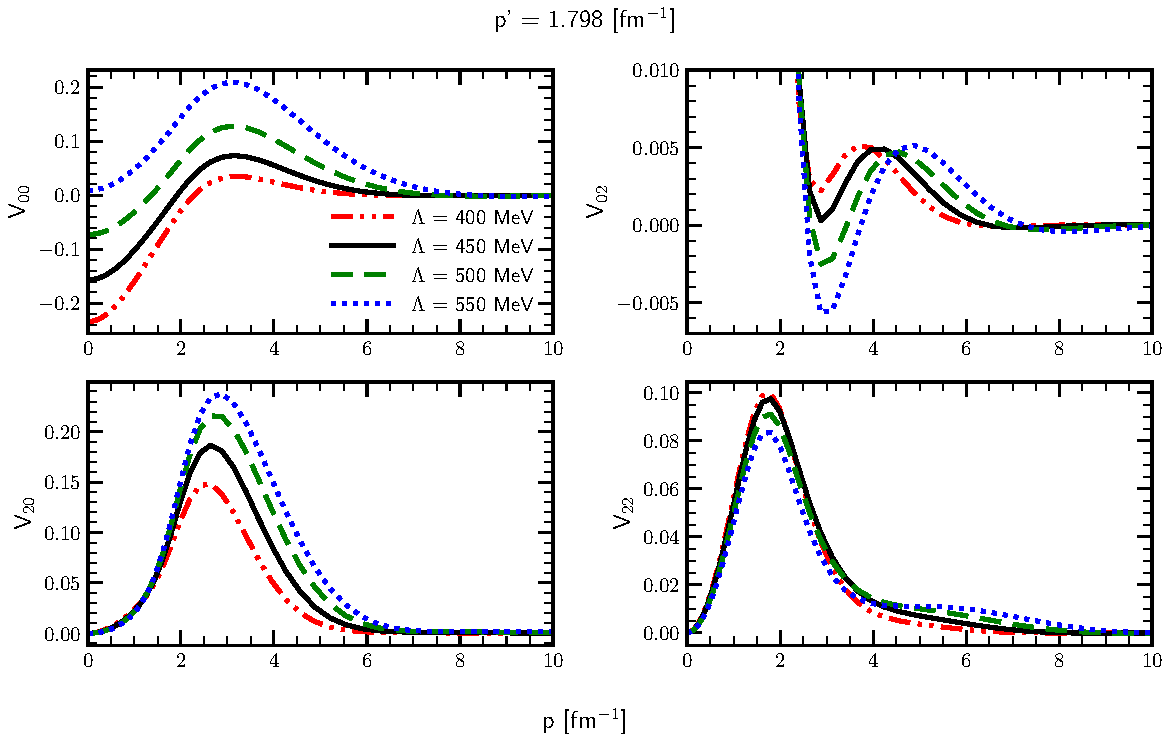
\includegraphics[width=0.95\textwidth]{PlotData/Deuteron/WAVEFUNC/potential_pp1.798.pdf}
    \end{center}
    \caption{Potential components as a function on the momentum $p$ with fixed
    value of the momentum $p'$=1.798 [fm?].
    }
    \label{potential_cutoff}
\end{figure}



The potential may be transformed from coordinate to momentum space (or vice versa),
but it is important at which frame the regularization was performed
and what was a regularization function. That's why there are different 
versions of chiral potential. One is \gls{scs} potential \cite{Epelbaum2014SCS}
and another one is similar, but with regularization applied in momentum space (\gls{sms} potential) \cite{reinkrebs2018}.


\subsection*{Currents}
 
% When it comes to the study of scattering processes on nuclei one has 
% to construct nuclear matrix elements, the crucial part 
% of which is nuclear current. The currents should be consistent with
% the force used


% \chapter{NN potentials}
\label{potentials}
\section{The OPE-Gaussian potential}
\label{OPEG-potential}
The OPE-Gaussian force is a phenomenological NN potential which has been presented by R. Navarro P{\' e}rez, J. E. Amaro, and E. Ruiz Arriola in 2014~\cite{NavarroPerez2014}. In usuall way, this potential can be decomposed to the short-range $V_{\mathrm{short}}(r)$ and the long-range $V_{\mathrm{long}}(r)$ parts,
\begin{equation}
V(r) = V_{\mathrm{short}}(r)\theta(r_{c} - r) + V_{\mathrm{long}}(r)\theta(r - r_{c})\;,
\end{equation}
\label{eq_31}
where $r$ is the internucleon distance and for the OPE-Gaussian potential $r_{c} =$ 3 fm.

The long-range force $V_{\mathrm{long}}(r)$ is, in turn, the sum of the one-pion exchange (OPE) force and the electromagnetic (EM) corrections:
\begin{equation}
V_{\mathrm{long}}(r) = V_{\mathrm{1\pi}} + V_{\mathrm{EM}}\;.
\label{eq_32}
\end{equation}
% the sum of the usual one-pion exchange potential (OPE), $V_{OPE}$, and the electromagnetic corrections for the proton-proton interaction, $V_{em}$.
The OPE potential $V_{\mathrm{1\pi}}$ is the same as the charge-dependent OPE potential used in the PWA93 by the Nijmegen group~\cite{Stoks1993} and the AV18 potential~\cite{Wiringa1995} which reads as
\begin{equation}
V_{\mathrm{\mathrm{1\pi}}}(r) \equiv V_{m, \mathrm{\mathrm{1\pi}}}(r) = \frac{1}{3}mf^{2}\left(\frac{m}{m_{s}}\right)^{2}\left[Y_{m}(r)\vec{\sigma}_{1}\cdot\vec{\sigma}_{2} + T_{m}S_{1,2}\right]\;,
\label{eq_33}
\end{equation}
where $\vec{\sigma}_{1}$ and $\vec{\sigma}_{2}$ denote the Pauli matrices of nucleons 1 and 2, respectively, $S_{1,2}$ is the tensor operator, and $Y_{m}(r)$ and $T_{m}(r)$ are the Yukawa and tensor functions,
\begin{equation}
\begin{split}
S_{12} &= 3\left(\vec{\sigma}_{1}\cdot\hat{r}~\vec{\sigma}_{2}\cdot\hat{r}\right) - \vec{\sigma}_{1}\cdot\vec{\sigma}_{2}\;,~\hat{r} = \frac{\vec{r}_{1} - \vec{r}_{2}}{\left|\vec{r}_{1} - \vec{r}_{2}\right|}\;, \\
Y_{m}(r) &= \frac{e^{-mr}}{mr}\;,\\
T_{m}(r) &= \frac{e^{-mr}}{mr}\left(1 + \frac{3}{mr} + \frac{3}{(mr)^{2}}\right)\;.
\end{split}
\label{eq_34}
\end{equation}
The scalling mass $m_s$ in Eq.~(\ref{eq_33}) is the charged-pion mass $m_{\pi^{\pm}}$, the average value of the pion mass $m = \frac{1}{3}(m_{\pi^{0}} + 2m_{\pi^{\pm}})$ = 138.057 MeV, $f = \sqrt{0.075} \approx 0.274$ is the pion coupling constant, for all pairs of nucleons ($pp$, $np$, $nn$). 
%and depends on a given pair of NN interactions ($pp$, $nn$, $np$) via pion exchange for the corresponding vertex of the Feynman diagram, i.e., $f_{pp\pi^{0}}$, $f_{nn\pi^{0}}$, $f_{np\pi^{-}}$ and $f_{pn\pi^{+}}$. According to PWA93, the Nijmegen group found that these coupling constants differ very little from each other, but due to charge symmetry\footnote{Charge symmetry is an approximate symmetry in which, if not take into account the electromagnetic force, then the interaction in the $nn$, $pp$, and $np$ pairs in the same quantum states are indistinguishable, and this, in turn, one can mean that the nuclear force can be considered as charge independent. Therefore, a proton and a neutron are considered as two states of one particle --- a nucleon.}~($f^{2}_{pp\pi^{0}} = -f_{nn\pi^{0}} f_{pp\pi^{0}}$) they were chosen approximately charge independent, i.e., $f^{2}_{pp\pi^{0}} = -f_{nn\pi^{0}} f_{pp\pi^{0}}= (f_{np\pi^{-}} f_{pn\pi^{+}})/\sqrt{2}\equiv f^{2} = 0.075$. 
As a result, charge dependence is yield only due to the difference between the charged $m_{\pi^{\pm}}$ and neutral $m_{\pi^{0}}$ pion mass and leads to
\begin{equation}
\begin{split}
V^{pp}_{\mathrm{\mathrm{1\pi}}}(r) &= V^{nn}_{\mathrm{1\pi}} \neq V^{np}_{1\pi}\;.\\  
%f^{2}_{p}V_{\mathrm{\mathrm{1\pi}}, m_{\pi^{0}}}(r)\; \\
%V^{np}_{\mathrm{\mathrm{1\pi}}}(r) &= -f^{2}_{0}V_{\mathrm{\mathrm{1\pi}}, m_{\pi^{0}}}(r) + (-1)^{T + 1}2f^{2}_{c}V_{\mathrm{\mathrm{1\pi}}, m_{\pi^{\pm}}}(r)\;,
\end{split}
\label{eq_35}
\end{equation}
%where $T$ is the total isospin of two nucleons and the following definitions
%\begin{equation}
%\begin{split}
%f^{2}_{p} &\equiv f_{pp\pi^{0}}f_{pp\pi^{0}}\;,~f^{2}_{n} \equiv f_{nn\pi^{0}}f_{nn\pi^{0}}\;, f^{2}_{p} = f^{2}_{n}\;,\\
%f^{2}_{0} &\equiv -f_{nn\pi^{0}}f_{pp\pi^{0}},~2f^{2}_{c}\equiv f_{np\pi^{-}}f_{pn\pi^{+}}\;.
%\end{split}
%\label{eq_351}
%\end{equation}
The EM corrections correspond to the $np$ and $pp$ potentials. The $np$ potential contains only a magnetic moment (MM) interaction 
\begin{equation}
V^{np}_{\mathrm{EM}} = V^{np}_{\mathrm{MM}}(r) = -\frac{\alpha\mu_{n}}{2m_{n}r^{3}}\left(\frac{\mu_{p}S_{1,2}}{2m_{p}} + \frac{\vec{L}\cdot\vec{S}}{\mu}\right)\;,
\label{eq_36}
\end{equation}
where $m_{n}$ and $m_{p}$ are the neutron and proton masses, $\mu$ is the reduced mass of the nucleon, $\mu_{n}$ and $\mu_{p}$ are the neutron and proton magnetic moments, $\vec{L}$ and $\vec{S}$ denote the angular momentum and spin operator, respectively, and $\vec{L}\cdot\vec{S}$ is the 2N spin-orbit operator. The $pp$ EM potential contains one- and two-photon exchange, vacuum polarization and a magnetic moment interaction
\begin{equation}
V^{pp}_{\mathrm{EM}} = V^{pp}_{\mathrm{C_{1}}}(r) + V^{pp}_{\mathrm{C_{2}}}(r) + V^{pp}_{\mathrm{VP}}(r) + V^{pp}_{\mathrm{MM}}(r)\;,
\label{eq_37}
\end{equation}
with detalied expressions given in Eqs. (9-12) of Ref.~\cite{Perez2013}
%\begin{equation}
%\begin{split}
%V^{pp}_{\mathrm{C_{1}}}(r) &= \frac{\alpha^{\prime}}{r}\;, \\
%V^{pp}_{\mathrm{C_{2}}}(r) &= \frac{\alpha\alpha^{\prime}}{M_{p}r^{2}}\;,\\
%V_{\mathrm{VP}}(r) &= \frac{2\alpha\alpha^{\prime}}{3\pi r}\int\limits_{1}^{\infty}e^{-2m_{e}rx}\left(1 + \frac{1}{2x^{2}}\right)\frac{\sqrt{x^{2} - 1}}{x^{2}}\mathrm{d}x\;,\\
%V^{pp}_{\mathrm{MM}} &= - \frac{\alpha}{4M^{2}_{p}r^{3}}\left[\mu^{2}_{p}S_{1,2} + 2(4\mu_{p} - 1)\vec{L}\cdot\vec{S}\right]\;.
%\label{eq_38}
%\end{split}
%\end{equation}
%All these potentials Eq.~(\ref{eq_38}) are used for distances $r_{c} \gtrsim$ 3 fm. It was also taken into account the energy dependence, expressed in terms of a parameter
%\begin{equation}
%\alpha^{\prime} = \alpha\frac{1 + \frac{2k^{2}}{M^{2}_{p}}}{\sqrt{1 + \frac{k^{2}}{M^{2}_{p}}}}\;,
%\end{equation}
%where $k$ is the center of mass momentum, $\alpha$ is the fine structure constant.

Below $r_{c}$ = 3 fm the short-range part $V_{short}(r)$ of the OPE-Gaussian force is built from 18 spin-isospin operators $\hat{O}_{n}$, 16 of these operators are the same as in the AV18 model~\cite{stoks1993partial}. Among them 14 operators are charge-independent,
%16 are the same as in the AV18 model, see~\cite{Wiringa1995}, the set of 14 operators are charge-independent, which are denoted as $c, \tau, \sigma, \sigma\tau, t, t\tau, ls, ls\tau, l2$, and are given by
\begin{equation}
\begin{split}
\hat{O}_{i\in\left[1, 14\right]} = &\lbrace\mathds{1}, \vec{\tau}_{1}\cdot\vec{\tau}_{2}, \vec{\sigma}_{1}\cdot\vec{\sigma}_{2}, (\vec{\sigma}_{1}\cdot\vec{\sigma}_{2})(\vec{\tau}_{1}\cdot\vec{\tau}_{2}), S_{12}, S_{12}(\vec{\tau}_{1}\cdot\vec{\tau}_{2}),\\ &\vec{L}\cdot\vec{S}, \vec{L}\cdot\vec{S}(\vec{\tau}_{1}\cdot\vec{\tau}_{2}), \!\vec{L}^{2}, \!\vec{L}^{2}(\vec{\tau}_{1}\cdot\vec{\tau}_{2}), \\ &\!\vec{L}^{2}(\vec{\sigma}_{1}\cdot\vec{\sigma}_{2}), \!\vec{L}^{2}(\vec{\sigma}_{1}\cdot\vec{\sigma}_{2})(\vec{\tau}_{1}\cdot\vec{\tau}_{2}), (\vec{L}\cdot\vec{S})^{2}, (\vec{L}\cdot\vec{S})^{2}(\vec{\tau}_{1}\cdot\vec{\tau}_{2})\rbrace\;.
\end{split}
\label{firspart}
\end{equation}
The remaining operators
\begin{equation}
\begin{split}
\hat{O}_{i\in\left[15, 18\right]} = &\lbrace T_{12}, (\vec{\sigma}_{1}\cdot\vec{\sigma}_{2}),  \!\vec{L}^{2}T_{12}, \!\vec{L}^{2}(\vec{\sigma}_{1}\cdot\vec{\sigma}_{2})T_{12}\rbrace\;,
%O_{i\in\left[15, 21\right]} = &\lbraceT_{12}, (\vec{\sigma}_{1}\cdot\vec{\sigma}_{1}), T_{12}S_{12}T_{12}, (\tau_{z1} + \tau_{z2}),\\&(\vec{\sigma}_{1}\cdot\vec{\sigma}_{2})(\tau_{z1} + \tau_{z2}), L^{2}T_{12}, L^{2}(\vec{\sigma}_{1}\cdot\vec{\sigma}_{2})T_{12}\rbrace\;,
\label{secondpart}
\end{split}
\end{equation}
with $T_{12} = 3\tau_{z1} \tau_{z2} - \vec{\tau}_{1}\cdot\vec{\tau}_{2}$ introduce charge dependence.
Each element of sets (\ref{firspart}-\ref{secondpart}) is multiplied by a sum of four Gaussian functions $F_{i, n}(r) = V_{i,n} exp(-r^{2}/(2a^{2}_{i}))$, where $a_{i} = \frac{a}{1 + i}$ and $V_{i,n}$ are the strength coefficients. Thus
\begin{equation} 
V_{\mathrm{short}}(r) = \sum_{n = 1}^{18}\hat{O}_{n}\left[\sum_{i = 1}^{4}V_{i, n}F_{i, n}(r) \right]\;.
\end{equation}
\begin{table}
\begin{center}
\begin{tabular}{|c|c|c|c|c|}
\hline
Operator &$V_{1, n}$& $V_{2, n}$& $V_{3, n}$ & $V_{4, n}$ 								   \\ \hline
$\mathds{1}$     	 & -19.28330126 & 126.28715008 & -648.61345585 & 694.49367435    \\ \hline
$\vec{\tau}_{1}\cdot\vec{\tau}_{2}$  	 & 2.36233395   &-25.47505195  & 130.03224633  &-284.71844492	   \\ \hline
$\vec{\sigma}_{1}\cdot\vec{\sigma}_{2}$     & 6.05581487   &-75.18832503  & 372.41961972  &-530.80008401    \\ \hline
$\tau\sigma$ & 7.36008330   &-48.55160272  &273.71591816   &-349.00547346    \\ \hline
$(\vec{\sigma}_{1}\cdot\vec{\sigma}_{2})(\vec{\tau}_{1}\cdot\vec{\tau}_{2})$& 1.99828652   &-22.12164190  &70.84584496    &-50.72248959     \\ \hline
$S_{12}, S_{12}(\vec{\tau}_{1}\cdot\vec{\tau}_{2})$& 15.02271531  & -38.34776035 & 183.80564790  & -160.48060286   \\ \hline
$\vec{L}\cdot\vec{S}$& -2.61725312  & 39.43014573  &-217.03270342  &-109.64162556    \\ \hline
$\vec{L}\cdot\vec{S}(\vec{\tau}_{1}\cdot\vec{\tau}_{2})$& 0.01009424   &2.59116238    &-26.57555840   &-77.56809604     \\ \hline
$\!\vec{L}^{2}, \!\vec{L}^{2}(\vec{\tau}_{1}\cdot\vec{\tau}_{2})$& 1.43519736   &-23.58906341  &67.86552330    &144.11773134     \\ \hline
$\!\vec{L}^{2}(\vec{\sigma}_{1}\cdot\vec{\sigma}_{2})$&-0.41138176   &8.33346137    &-82.98819447   & 175.09618737    \\ \hline
$\!\vec{L}^{2}(\vec{\sigma}_{1}\cdot\vec{\sigma}_{2})(\vec{\tau}_{1}\cdot\vec{\tau}_{2})$&-0.09972181   &2.25339230    &-51.87819771   &175.08890636 	   \\ \hline
$(\vec{L}\cdot\vec{S})^{2}$&-0.26615545  &6.63257735    &-55.34306118   &100.71528331 	   \\ \hline
$(\vec{L}\cdot\vec{S})^{2}(\vec{\tau}_{1}\cdot\vec{\tau}_{2})$&0.46072934   &-11.65544792   &150.58275714   &-302.07573779    \\ \hline
$ls2\tau$    &0.71538487   &-18.88652666   &141.73160452   &-182.73368764    \\ \hline
$T_{12}$&0.63788724   &-7.90421846    &24.23180376    &-19.73899169      \\ \hline
$(\vec{\sigma}_{1}\cdot\vec{\sigma}_{2})$   &-0.63788724  &7.90421846     &-24.23180376   &19.73899169       \\ \hline
$ \!\vec{L}^{2}T_{12}$&-0.10631454  &1.31736974     &-4.03863396    &3.28983195        \\ \hline
$ \!\vec{L}^{2}(\vec{\sigma}_{1}\cdot\vec{\sigma}_{2})T_{12}$ &0.10631454   &-1.31736974    &4.03863396     &-3.28983195       \\ \hline
%$r_{c}$      &2.30347728   &				& 				 &					\\ \hline
\end{tabular}
\caption{The central values of operator coefficients $V_{i, n}$ (in MeV) of the OPE-Gaussian potential. The parameter $a$ is 2.30347728 [fm].}
\label{tableOPEG}
\end{center}
\end{table}
It should be noted that in Ref.~\cite{NavarroPerez2014} there are 21 operators, but three of them ($tT$, $\tau_{z}$ and $\sigma\tau_{z}$) are almost equal zero in practical calculations~\cite{NavarroPerez2014},~\cite{privateArriola} and have been skipped in the final version of the OPE-Gaussian potential. The free parameter $a$, which determines the width of the functions $F_ {i, n}(r)$, together with the operator coefficients $V_ {i, n}$ were fixed from the data NN collected in Granada-2013 database~\cite{Perez2013}.
%, see Table~\ref{tableOPEG}. 

The construction of this database was done in the following steps:
\begin{enumerate}
\item The Granada group collected 8124 available $np$- and $pp$-scattering data taken between 1950 and 2013 in the laboratory energy range $E_{\mathrm{lab}}$ up to 350 MeV. They removed data with unknown or unclear statistical and systematic uncertainties.
\item They performed the least-squares fitting procedure to this database and the deuteron binding energy by the coarse-grained potential and delta-shell representation for the short and intermediate part of the NN interaction in terms of partial-wave decomposition at given scattering energy and angle~\cite{Perez2013, NavarroPerez2015}. 
%After the fitting procedure, the $\chi^{2}$ is calculated and minimized with respect to the fitted potential parameters of the $\delta$-shell potential.
%In addition, they normalized data as an additional contribution to the $\chi^{2}$ based on the proposed idea by Gross and Stadler in Ref.~\cite{gross2008covariant}.  
%\item They performed the least-squares fitting procedure for $np$ scattering below pion production threshold by the coarse-grained potential and delta-shell representation ($\delta$-shell potential) for the short and intermediate part of the NN interaction~\cite{perez2013partial, Perez2013, NavarroPerez2015}. After the fitting procedure, the $\chi^{2}$ is calculated and minimized with respect to the fitted potential parameters of the $\delta$-shell potential.
\item Some sets of data were incompatible with each other. To remove them, R. Navarro P{\' e}rez and collaborators applied the 3$\sigma$-criterion introduced by the Nijmegen group in the PWA93. Namely, for the Gaussian statistical data uncertainties $\Delta O^{data}_{i}$, the residuals for observables $O_{i}$, $\left(O^{data}_{i} - O^{theory}_{i}\right)/\Delta O^{data}_{i}$ should be normal-distributed within a  3$\sigma$-confidence level. Unfortunately, this criterion has disadvantages. One of them is that when non-normal outliers data is rejected, it leads to a significantly improved fitting of compatible data (overestimation)~\cite{Perez2013}. Therefore, they applied the improved 3$\sigma$-criterion~\cite{Perez2013} to the complete database based on the idea of 3$\sigma$ self-consistent rejection given by Gross and Stadler~\cite{gross2008covariant} and again refitted of the parameters. As a result, they obtained the new database (the 3$\sigma$ self-consistent Granada-2013 database), that incorporates 6713 $pp$ and $np$ data and confirmed good statistical properties of their $\chi^{2}$ fit with the value of $\chi^{2}$/datum = 1.05.
%~\footnote{It should be noted that the $\chi^{2}$/datum value is given by $\chi^{2}/N_{\mathrm{dof}}$, where $N_{\mathrm{dof}} = N - P$ is the number of degrees of freedom depending on the number of data, $N$, and the number of parameters, $P$. $N = N^{\mathrm{exp}}_{data} + N^{\mathrm{norm}}_{data}$, where $N^{\mathrm{exp}}_{data}$ is the number of data points and $ N^{\mathrm{norm}}_{data}$ the number of estimated normalizations.}.
Having the database and emerging phase-shifts it was possible to fix 42 free partial-wave parameters of the OPE-Gaussian potential which are linear functions of operator coefficients $V_{i, n}$~\cite{NavarroPerez2014}. Final, used also in this thesis, values of $V_{i,n}$ are presented in Table~\ref{tableOPEG}. The resulting $\chi^{2}$/datum for the OPE-Gaussian force amounts 1.06 as fitted to data listed in Ref.~\cite{Perez2013}. The performed extensive statistical analysis of data and careful fitting procedures allowed authors of Ref.~\cite{Perez2014} to provide not only the values of free parameters but also their covariance matrix~\cite{Perez2014}. 
%Using this matrix they sampled from the multivariate normal distribution the free parameters $V_{i, n}$ and $a$, and computed their uncertainty~\cite{Perez2014}.
\end{enumerate}
%We have been equipped by the authors of Ref.~\cite{NavarroPerez2014} with a sample of 50 sets of potential coefficients $\lbrace V_{i, n}\rbrace$ and its the central values with their uncertainties, which a little differ from values in paper~\cite{NavarroPerez2014} in given in Table. 
The knowledge of the covariance matrix of parameters allowed authors of Ref.~\cite{Perez2014} to sample, from the multivariate normal distribution another sets of potentials parameters. They provided us with a sample of 50 sets of parameters $\lbrace V_ {i, n}, a\rbrace$ and its central values. Finally, we would like to note, that the OPE-Gaussian potential has a similar structure to the AV18 force and thus it can be regarded as a remastered version of the standard AV18 model. 

% which can be by the formula
%\begin{equation}
%R_{i} = \frac{O^{exp}_{i}-O^{th}_{i}}{\Delta O^{exp}_{i}}
%\end{equation}

\section{The chiral SMS potential}
\label{chiral_model}
%In Chapter~\ref{introduction}, I outlined that the effective field theory of QCD is $\chi$EFT. which is constructed for systems with a separation of scales based on a power con
Choosing nucleons and pions as only particles in the theory the chiral NN potential can be written as
\begin{equation}
V_{2N} =  V_{\mathrm{cont}} + V_{\mathrm{\pi}}
\label{eg:ch1}
\end{equation}
where $V_{\mathrm{cont}}$ is the contact interaction between nucleons and $V_{\pi}$ represents the pion contributions to the two-nucleon potential. The long-range part of nuclear forces is completely determined
by the chiral symmetry of QCD and experimental information on pion-nucleon ($\pi$N) scattering. Moreover, the pion exchange contributions can be separated by the number of exchanged pions at each chiral order of the chiral expansion, i.e.
\begin{equation}
\begin{split}
&V_{1\pi} = V^{(0)}_{1\pi} + V^{(2)}_{1\pi} + V^{(3)}_{1\pi} + V^{(4)}_{1\pi} + V^{(5)}_{1\pi} + \ldots\;,\\
&V_{2\pi} = V^{(2)}_{1\pi} + V^{(3)}_{1\pi} + V^{(4)}_{1\pi} + V^{(5)}_{1\pi} + \ldots\;.
\end{split}
\label{eg:ch2}
\end{equation}
As an example I show the OPE potential at order $Q^{0}$ (LO) given directly in momentum space reads
\begin{equation}
V^{(0)}_{1\pi}(\vec{q}) = -\left(\frac{g_{A}}{2F_{\pi}}\right)\vec{\tau}_{1}\cdot\vec{\tau}_{2}\frac{\vec{\sigma}_{1}\cdot\vec{q}~\vec{\sigma}_{2}\cdot\vec{q}}{q^{2} + m^{2}_{\pi}}\;.
\end{equation}
Here $\vec{q}$ is the relative momentum transfer of the exchanged pion $\vec{q} = \vec{p}^{~\prime} - \vec{p}$, $\vec{p}$ and $\vec{p}^{~\prime}$ are the initial and final relative momenta of the two nucleons in the c.m.s, $\vec{\tau}_{1}$, $\vec{\tau}_{2}$ denote isospin matrices of nucleons 1 and 2, respectively. $g_{A}$ = 1.29 is the pion-nucleon axial coupling constant and $F_{\pi}$ = 92.4 MeV is the pion decay constant. 

Similarly, the contact interaction between nucleons, which plays a role of the short-range part of the NN force takes the form
\begin{equation}
\begin{split}
&V_{\mathrm{cont}} = V^{(0)}_{\mathrm{cont}} + V^{(2)}_{\mathrm{cont}} + V^{(4)}_{\mathrm{cont}} \ldots\;.
\end{split}
\label{eg:ch3}
\end{equation}
The chiral potential with semilocal regularization in momentum space (the SMS potential) has been derived completely up to the fifth-order (N$^{4}$LO) of the chiral expansion by the Bochum-Bonn group~\cite{Reinert2018}. Comparing the previous chiral forces, the authors fixed the $\pi$N low-energy constants (LECs) using the Roy-Steiner analysis~\cite{hoferichter2015matching}, skipped redundant contact terms in the higher order of the chiral expansion (starting at order $Q^{4}$, i.e. N$^{3}$LO), and, using the Granada-2013 database, determined adjustable parameters of the potential from $np$ and $pp$ scattering data and the deuteron binding energy. They also added the four leading contact terms acting in the N$^{5}$LO ($Q^{6}$ order) F-waves from Ref.~\cite{Entem2017} to their N$^{4}$LO, potential obtaining so-called N$^{4}$LO$^{+}$ interaction.
%as a result, they got updated potential as N$^{4}$LO$^{+}$. 
%For example, the chiral expansion of the NN forces at the leading order is visualized schematically in Figure~\ref{LO}.
%\begin{figure}[h]
%\begin{center}
%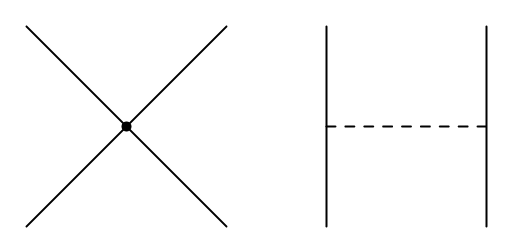
\includegraphics[width=0.5\textwidth]{PhD-text/3_Potentials/LO.png}
%\end{center}
%\caption{The structure of the chiral NN force at the LO order. Solid and dashed lines represent nucleons and pions, respectively.}
%\label{LO}
%\end{figure}
%Implementing local regularization in momentum space~\cite{Reinert2018} the potential $V_{\mathrm{\mathrm{1\pi}}, \Lambda}(m_{\pi})$  
%\begin{equation}
%V_{\mathrm{\mathrm{1\pi}}, \Lambda}(m_{\pi}, \vec{q}) = -\frac{g^{2}_{A}}{4F^{2}_{\pi}}
%\left(\frac{\vec{\sigma}_{1}\cdot\vec{q}~\vec{\sigma}_{2}\cdot\vec{q}}{m^{2}_{\pi} + q^{2}} + C(m_{\pi})~\vec{\sigma}_{1}\cdot\vec{\sigma}_{2}\right)e^{-\frac{m^{2}_{\pi} + q^{2}}{\Lambda^{2}}}\;,
%\end{equation}
%where the constant $C_{\pi}$ depends on the spin-spin part and reads as
%\begin{equation}
%C_{m_{\pi}} = -\frac{\Lambda\left(\Lambda^{2} - 2 m^{2}_{\pi}\right) + 2\sqrt{\pi}m^{3}_{\pi}e^{m^{2}_{\pi}/\Lambda^{2}}\mathrm{erfc}\left(\frac{m_{\pi}}{\Lambda}\right)}{3\Lambda^{3}}\;,
%\end{equation}
%with the error function $\mathrm{erfc}(x)$
%\begin{equation}
%\mathrm{erfc}(x) = \frac{2}{\sqrt{\pi}}\int\limits_{x}^{\infty}e^{-t^{2}}\mathrm{dt}.
%\end{equation}

A general structure of the contact interactions of the chiral SMS force up to fourth-order (N$^{3}$LO) $Q^{4}$ is 
\begin{equation}
\begin{split}
&V^{(0)}_{\mathrm{cont}} = C_{S} + C_{T}\vec{\sigma}_{1}\cdot\vec{\sigma}_{2}\;,\\
&V^{(2)}_{\mathrm{cont}} = C_{1}q^{2} + C_{2}k^{2} + \left(C_{3}q^{2} + C_{4}k^{2}\right)\left(\vec{\sigma}_{1}\cdot\vec{\sigma}_{2}\right) + \frac{i}{2}C_{5}\left(\vec{\sigma}_{1}\cdot\vec{\sigma}_{2}\right)\cdot\left(\vec{k}\times\vec{q}\right)\\
&~~~~~~~~~+ C_{6}\left(\vec{q}\cdot\vec{\sigma}_{1}\right)\left(\vec{q}\cdot\vec{\sigma}_{2}\right) + C_{7}\left(\vec{k}\cdot\vec{\sigma}_{1}\right)\left(\vec{k}\cdot\vec{\sigma}_{2}\right)\;,\\
&V^{(4)}_{\mathrm{cont}} = D_{1}q^{4} + D_{2}k^{4} + D^{3}q^{2}k^{2} + D_{4}\left(\vec{q}\times\vec{k}\right)^{2}\\
&~~~~~~~~~+\left(D_{5}q^{4} + D_{6}k^{4} + D_{7}q^{2}k^{2} + D_{8}\left(\vec{q}\times\vec{k}\right)^{2}\right)\left(\vec{\sigma}_{1}\cdot\vec{\sigma}_{2}\right)\\
&~~~~~~~~~+\frac{i}{2}\left(D_{9}q^{2} + D_{10}k^{2}\right)\left(\vec{\sigma}_{1} + \vec{\sigma}_{2}\right)\cdot\left(\vec{k}\times\vec{q}\right)\\
&~~~~~~~~~+\left(D_{11}q^{2} + D_{12}k^{2}\right)\left(\vec{\sigma}_{1}\cdot\vec{q}\right)\left(\vec{\sigma}_{2}\cdot\vec{q}\right)\\
&~~~~~~~~~+\left(D_{13}q^{2} + D_{14}k^{2}\right)\left(\vec{\sigma}_{1}\cdot\vec{q}\right)\left(\vec{\sigma}_{2}\cdot\vec{q}\right)\\
&~~~~~~~~~+D_{15}\vec{\sigma}_{1}\cdot\left(\vec{q}\times\vec{k}\right)\vec{\sigma}_{2}\cdot\left(\vec{q}\times\vec{k}\right)\;,
\end{split}
\end{equation}
%Short-range interactions have to be tuned to experimental data. 
where $\vec{k} = (\vec{p} + \vec{p}^{~\prime})/2$ and $C_{S}$, $C_{T}$ $C_{1,\ldots, 7}$ and $D_{1,\ldots, 15}$ are the LECs which determine the strength of short-range interaction and should be find from data. 

The usage of nuclear forces derived from $\chi$EFT in few- and many-body problems demand a local regularization for the pion exchange contributions to reduce the amount of finite-cutoff terms and to avoid divergences after substituting, e.g., into the Lippmann-Schwinger equation. In Ref.~\cite{Epelbaum2015}, the Bochum-Bonn group implemented the regularization of the long-range potential in coordinate space, see Eq.~\ref{reg_coord}. Although such regulator allowed to significantly reduce the long-range cutoff terms, but its application turned out to be difficult for the regularization of 3NFs and currents at higher orders of chiral expansion. 
Therefore, the Bochum group introduced a local regularization scheme of long-range forces in momentum space by emplyoing a regularization of static one-pion exchange contribution~\cite{Reinert2018} in the following way
\begin{equation}
f(p^{\prime}, p) \propto \exp\left(-\frac{\left(m^{2}_{\pi} - \!\vec{\,q}^{2}\right)^{2}}{\Lambda^{2}}\right)\;,
\end{equation}
with the cutoff values of $\Lambda = 400, 450, 550$, and 550 MeV. Such approach, as the authors of Ref.~\cite{Reinert2018} argue contributes only to the short-range terms and does not influence the long-range pion exchange potentials.

Implementing local regularization to the long-range potential and multiplying the contact terms with a non-local Gaussian regulator $\mathrm{exp}\left(-\frac{p^{\prime 2} + p^{2}}{\Lambda^{2}}\right)$ in combination with the very detailed fitting procedure of the NN contact LECs leads to a high-quality potential. Specifically, for the chiral SMS potentials of Ref.~\cite{Reinert2018} obtained with the Granada-2013 database~\cite{NavarroPerez2014} the covariance matrices of its free parameters (LECs) at all chiral orders LO-N$^{4}$LO$^{+}$ have been obtained. The number of free parameters (LECs) is 2, 9, 9, 22, 23, 27 at LO, NLO, N$^{2}$LO, N$^{3}$LO, N$^{4}$LO and N$^{4}$LO$^{+}$, respectively. 
Sample visualization of correlations among the various LECs is given in Figure 10 of Ref.~\cite{Reinert2018} for the chiral N$^{4}$LO$^{+}$ SMS potential with $\Lambda$ = 450 MeV. 

Currently, the chiral SMS NN potential is the interaction delivering the best description of NN data. For example, the SMS N$^{4}$LO$^{+}$ with regularization parameter $\Lambda$ = 450~MeV gives $\chi^{2}$/datum = 1.06 ($np$ scattering data) and $\chi^{2}$/datum = 1.00 ($pp$ scattering data), see Table 4 of Ref.~\cite{Reinert2018} up to 300 MeV. In addition, the availability of covariance matrices of LECs for all chiral cutoffs and orders allows us to study, for the first time for a chiral force, the propagation of uncertainties of NN interaction parameters to 3N continuum observables, see Chapter~\ref{application_cov_mat} and Chapter~\ref{error}. 
%~\cite{Reinert2018} the potential $V_{\mathrm{\mathrm{1\pi}}, \Lambda}(m_{\pi})$ 




% \chapter{Application of a covariance matrix}
\label{application_cov_mat}
In Chapter~\ref{introduction}, I have outlined the advantages of using the covariance matrix of NN potential parameters and briefly mentioned types of errors to the Nd scattering observables. In this chapter I discuss the various sources of theoretical uncertainties in the \textit{ab initio} type calculations based on the chiral SMS model at various orders, neglecting the 3N force present in describing the 3N processes. The main results of such study were previously shown in our Refs.~\cite{Skibinski2018, volkotrub2020uncertainty}. Studies of correlations among all calculated 2N and 3N observables, as well as between observable and specific potential parameters, will also be discussed.

\section{Uncertainty quantification presented in 3N studies}
\label{uq}

\subsection{Determination of statistical uncertainty in a 3N system}
\label{statistical}
As defined in Chapter~\ref{introduction}, the statistical uncertainty refers to an error arising from uncertainties of parameters of a given NN interaction. In our method of estimation, computation of the statistical uncertainties requires a big sample of predictions obtained with different sets of parameters within one model of interaction. 
%A key element in obtaining the magnitudes of statistical uncertainties is the covariance matrix (or equivalently the correlation matrix) of free parameters as repeatedly mentioned, is available for the SMS chiral potential of Ref.~\cite{Reinert2018} and the OPE-Gaussian potential of Ref.~\cite{NavarroPerez2014}. 

%In Ref.~\cite{Skibinski2018} we described our method how to propagate theoretical uncertainties from NN force to 3N scattering observables in the case of the OPE-Gaussian potential. 
The algorithm for determining statistical uncertainty and using it further for the chiral SMS force can be divided into the following steps:
%Drawing on our procedure of determining the theoretical uncertainty arising from the NN potential parameters, which was described in ~\cite{Skibinski2018}, the statistical uncertainty can be found by the following steps:
\begin{enumerate}
\item Preparation of sets of the potential parameters.

Having at our disposal covariance matrix for the potential parameters, as well as central values of parameters, I sample 50 sets of the potential parameters from the multivariate normal distribution. The multivariate sampling was done using the Mathematica\textsuperscript{\textregistered}~\cite{Mathematica11p3} computing system (see Appendix~\ref{appendix_1}). Such a number of sets guarantee a statistically meaningful probe, as will be shown in Chapter~\ref{error}. 
%Being in contact with the Bochum-Bonn group we received one set $S_{0}$ of central values and the covariance matrices of LECs for all orders of the chiral expansion.
%50 covariance matrices for all orders of the chiral expansion of the OPE-Gaussian potential parameters, sampled from the multivariate normal distribution (in space of parameters) with known expectation values and covariance matrix, and one set of expectation values of potential parameters $S_{0}$, see Ref.~\cite{Skibinski2018}. 
%($S_i$ with $i = 1,  \ldots, 50$)
%
%In the case of the chiral SMS potentials from the Bochum group we have been equipped by the set $S_{0}$ and the covariance matrices for all orders of the chiral expansion.   
%The potential parameters for the chiral interaction result from $\chi^{2}$ fitting of theoretical predictions directly to the data collected in the Granada database~\cite{Perez2013}. The fitting procedure is described in detail in Refs.~\cite{Reinert2018} and~\cite{ReinertMaster}. As a result, 
%the central values of the parameters and their covariance matrix are obtained. Being in contact with members of the Bochum-Bonn group we received the set ($S_{0}$) of expectation values and the covariance matrices of potential parameters for all orders of chiral expansion. The various sets of potential parameters have been computed by sampling from the multivariate normal distribution (in space of parameters) with a given covariance matrix. As a result, we sampled 50 sets ($S_{i}, i = 1 \ldots 50)$ of NN potential parameters. Also in the case of the OPE-Gaussian interaction, we are already in contact with authors of this potential and have been equipped by them with the set of the central values of the parameters and a sample of 50 sets of potential parameters. 
\item Computing observables for each set of potential parameters

For each set $S_{i}$ $(i = 0,1, \ldots, 50)$ %I calculated the deuteron wave-function and the $t$ matrix, solved, at
%each considered energy, the Faddeev equation to construct the transition amplitude from which the 3N observables can be obtained for all investigated models of NN interaction. 
I computed the deuteron wave-function by solving the Schr{\"o}dinger equation and the $t$-matrix elements from the Lippman-Schwinger equation and solved the Faddeev equation to construct the transition amplitude from which the 3N observables can be obtained for all investigated models of NN interaction. From solutions of the Lippmann-Schwinger equation 2N observables can be also computed. More details about these calculations will be given in Chapter~\ref{formalism}. As a result, the angular dependence of various 3N scattering observables is known for each set of parameters $S_{i}$. The obtained predictions can be used to study
%by solving the Schr{\"o}dinger equation in momentum space. In this case Schr{\"o}dinger equation can be expressed as an eigenvalue problem. The solutions of this problem -- eigenvalue which corresponds to the binding energy and corresponding eigenvector which can be directly linked to the deuteron wave function -- were obtained using the standard numerical methods~\cite{numrecipesFortran} and the LAPACK library. 
\begin{enumerate}[label=(\alph*)] % (a), (b), (c), ...
\item for a given observable $X$ at an energy $E$ and at a scattering angle $\theta$, the empirical probability density function of the observable $X$($E$, $\theta$) resulting when various sets $S_i$, ($i = 1, \ldots, 50$) are used;
\item for a given observable $X$, both the angular and energy dependencies of results based on various sets $S_{i}$.
\end{enumerate}
This, in turn, allows one to find the magnitude of statistical uncertainty of a given 3N observable $X$ and to analyze correlations among all observables. 

\item Quantification of the statistical uncertainty 

Various estimators can be used to quantify the statistical uncertainty of the observable $X(E, \theta$). 
For example, by assuming there are 50 sets of potential parameters: 
\begin{enumerate}[label=(\alph*)]
\item The sample standard deviation $\sigma (X) = \sqrt{\frac{1}{50-1}\sum\limits_{i = 1}^{50}\left(X_{i}(E,\theta) - \bar{X}(E, \theta)\right)^{2}}$, where $\bar{X}(E, \theta)$ is the mean value of predictions.
\item $\frac{1}{2}\Delta_{100\%} \equiv \frac{1}{2}\left(\max\lbrace X_{i}(E, \theta)\rbrace - \min\lbrace X_{i}(E, \theta)\rbrace \right)$, where the minimum and maximum are taken over all predictions $\lbrace X_{i}(E, \theta)\rbrace$ based on 50 sets of LECs $S_{i}, i = 1, 2, \ldots, 50$.
\item $\frac{1}{2}\Delta_{68\%} \equiv \frac{1}{2}\left(\max\lbrace X_{i}(E, \theta)\rbrace - \min\lbrace X_{i}(E, \theta)\rbrace \right)$, where the minimum and maximum are taken over 34 (68\% of 50) predictions based on different sets of LECs. The set of 34 observables is constructed by discarding the 8 lowest and the 8 highest
predictions for a given observable and at specific scattering angle and energy.
\item $\frac{1}{2}$IQR: half of the standard estimator of the interquartile range being the difference between the third and the first quartile IQR = $Q_{3} - Q_{1}$. For the sample of size 50, this corresponds to taking half of the difference between the predictions on 37th and 13th positions in a sample sorted in ascending order. 
\end{enumerate}
\end{enumerate}
% and will be discussed in Section~\ref{stat} of Chapter~\ref{formalism}. The optimal estimator of the statistical uncertainty of the observable $O$($E$, $\theta$) at given energy and a scattering angle is calculated by the formula
%\begin{equation}
%\frac{1}{2}\Delta_{68\%} \equiv \frac{1}{2}\left(\max\lbrace O_{i}(E, \theta)\rbrace - \min\lbrace O_{i}(E, \theta)\rbrace \right)\;,
%\end{equation}
%where where the minimum and maximum are taken over 34 (68\% of 50) predictions based on 50 sets of the NN potential
%parameters. The set of 34 observables is constructed by discarding the 8 lowest and the 8 highest
%predictions for the observable $O$($E$, $\theta$). 
%The computation of the 2N scattering observables requires a calculation of the transition amplitude between initial and final two-nucleon states. The amplitude is given as the matrix element of the $t$-operator, which is a solution of the Lippmann-Schwinger equation. Thus during this step, we solved, again for each of the investigated models of interaction and all sets of parameter values, this equation and after the suitable anti-symmetrization, the transition amplitude and the observables were computed~\cite{glockle1983quantum, Glockle1996}.  
The estimators $\frac{1}{2}\Delta_{100\%}$ and $\sigma(X)$ are sensitive to possible outliers in the sample, and thus accepting them as estimators of dispersion can lead to overestimation of the statistical uncertainty. On the other hand, due to the fact that the IQR is calculated using only half of the elements in the sample can leads to an underestimation of the theoretical uncertainty. Therefore, we chose $\frac{1}{2}\Delta_{68\%}$ as an optimal measure for dispersion of predictions and consequently as an estimator of the statistical uncertainty~\cite{Skibinski2018}. 

%compare its size with the statistical uncertainties already obtained
\subsection{Determination of truncation errors within EKM method}
\label{truncation}
In addition to the statistical uncertainties, also the truncation errors, which play the role of systematic uncertainty can be evaluated. As was outlined in Chapter~\ref{introduction}, the truncation errors are uncertainties that arising from restriction to a given order of the chiral expansion. The one way to evaluate truncation errors is using the EKM approach~\cite{Epelbaum2015}. 
Consider any 3N scattering observable $X$ which can be expanded up to the $k$-th order of the chiral expansion $Q^{k}$ ($k = 0, 2, 3, \ldots$) but at a fixed cutoff value $\Lambda$ in the form
\begin{equation}
X = X^{(0)} + \Delta X^{(0)} + \Delta X^{(2)} + \Delta X^{(3)} + \ldots + \Delta X^{(k)}\;,
\label{eq:trunc1}
\end{equation}
where $\Delta X^{(2)} := X^{(2)} - X^{(0)}$, $\Delta X^{(k)} := X^{(k)} - X^{(k-1)}$ with $k > 2$, and $X^{(k)}$ is a prediction obtained at order $Q^{k}$.

The truncation error $\delta (X)^{(k)}$ of an observable $X$ at $k$-th order of the chiral expansion with $k = 0, 2, \ldots$ can be estimated as
\begin{equation}
\begin{split}
&\delta (X)^{(0)} \geq \max\left(Q^{2}|X^{(0)}|\right)\;,\\
&\delta (X)^{(2)} \geq \max\left(Q^{3}|X^{(0)}|, Q|X^{(2)} - X^{(0)}|\right)\;,\\
&\delta (X)^{(k)} \geq \max\limits_{2\leq j \leq k}\left(Q^{k+1}|X^{(0)}|, Q^{k+1-j}|\Delta^{(j)}|\right)~\mathrm{for}~j \geq 2\;,
\end{split}
\label{eq:trunc2}
\end{equation}
with the additional constraints $\delta (X)^{(2)} \geq Q\delta (X)^{(0)}$ and $\delta (X)^{(k)} \geq Q\delta (X)^{(k - 1)}$ for $k \geq 3$ are imposed on the truncation errors. 
The chiral expansion parameter $Q$ is
\begin{equation}
Q = \max\left(\frac{p}{\Lambda_{b}}, \frac{m_{\pi}}{\Lambda_{b}}\right)\;.
\label{eq:trunc3}
\end{equation}
In my calculations the breakdown scale of the chiral expansion $\Lambda_{b}$ was choosen as $\Lambda_{b}$ = 600~MeV based on the results from Refs~\cite{binder2016few, binder2018few} with the physical pion mass $m_{\pi}$ and the c.m.s. momentum $p$ corresponding to the considered incoming-nucleon laboratory $E_{\mathrm{lab}}$.
\subsection{The truncation errors with a given Bayesian model}
\label{bayes}
Since the EKM approach does not provide a statistical interpretation of the alleged uncertainties, we apply also the Bayesian approach to estimate truncation error. The authors of Refs.~\cite{Furnstahl2015, melendez2017bayesian} developed the Bayesian method to calculate the posterior probability distribution of truncation errors in $\chi$EFT for the $np$ total cross section at selected energies by applying the chiral NN potentials from Ref.~\cite{Epelbaum2015}. Within the LENPIC project the Bayesian model of Ref.~\cite{melendez2017bayesian} was slightly modified to study truncation errors not only in NN but also in 3N scattering,~\cite{epelbaum2020towards}. The same Bayesian procedure was already used in Ref.~\cite{volkotrub2020uncertainty}.

This Bayesian procedure determining the truncation errors was based on rewriting Eq. (\ref{eq:trunc1}) in terms of dimensionless expansion coefficients $c_{k}$ in the form
\begin{equation}
\begin{split}
X &= X^{(0)} + \Delta X^{(2)}+ \Delta X^{(3)}+ \Delta X^{(4)}+\ldots + \Delta X^{(k)} +\ldots \\&= X_{\mathrm{ref}}\left(c_{0} + c_{2}Q^{2} + c_{3}Q^{3} + c_{4}Q^{4} + \ldots\right)\;,
\end{split}
\label{eq:trunc4}
\end{equation}
where $\Delta X^{(k)}$ are the same as in Eq. (\ref{eq:trunc2}) and the dimensionless expansion coefficients $c_{k}$ are
\begin{equation}
c_{k} = \frac{X^{(k)} - X^{(k-1)}}{X_{\mathrm{ref}}Q^{k}}\;.
\end{equation}
The overall scale $X_{\mathrm{ref}}$ is
\begin{equation}
  X_{\mathrm{ref}} =
  \begin{cases}
    \max\left(\vert X^{(0)}\vert, Q^{-2} \vert \Delta X^{(2)}\vert \right)  & \text{for $k = 2$}\;, \\
    \max\left(\vert X^{(0)}\vert, Q^{-2} \vert \Delta X^{(2)}\vert, Q^{-3} \vert \Delta X^{(3)}\vert \right) & \text{for $k \geq 3$}\;,
  \end{cases}
\label{eq:trunc5}
\end{equation}
assuming that $\Delta X^{(i)}$ are known explicitly up to the $k = 3$. One can estimate the size of the truncation error at the k-th order of chiral expansion as $\delta X^{(k)}_{Bayes} \equiv X_{ref}\Delta$ where 
$\Delta \equiv \sum^{\infty}_{i = k + 1}c_{i}Q^{i} \approx \sum^{k + h}_{i = k + 1}c_{i}Q^{i}$ is distributed, 
given the knowledge of $\left\lbrace c_{i \leq k}\right\rbrace$
with a posterior probability density function
\begin{equation}
\text{pr}_{h}\left(\Delta\mid \left\lbrace c_{i \leq k} \right\rbrace \right) = \frac{\int^{\infty}_{0}d\bar{c}~\text{pr}_{h}\left(\Delta\mid\bar{c} \right)\text{pr}(\bar{c})\prod_{i \in A}\text{pr}(c_{i}\mid\bar{c})}{\int^{\infty}_{0}d\bar{c}~\text{pr}(\bar{c})\prod_{i \in A}\text{pr}(c_{i}\mid\bar{c})}\;.
\label{eq_posterior1}
\end{equation}
Here the prior probability density function $\text{pr}(c_{i}\mid\bar{c})$ is taken in form of a Gaussian N(0,$\bar{c}^2$) function 
and $\text{pr}(\bar{c})$ is a log-uniform distribution in range $(\bar{c}_{<},\bar{c}_{>})$.
Set $A$ is defined as 
$A = \left\lbrace n \in \rm{N}_{0} \mid n \leq k~\wedge~n \neq 1 \wedge n \neq m \right\rbrace $, $m \in  \left\lbrace 0, 2, 3 \right\rbrace$ and 
\begin{equation}
\text{pr}_{h}(\Delta\mid\bar{c}) \equiv \left[\prod^{k + h}_{i = k + 1}\int^{\infty}_{\infty}dc_{i}\text{pr}(c_{i}\mid\bar{c}) \right] \delta\left[\Delta - \sum^{k + h}_{j = k + 1}c_{j}Q^{j} \right]\;,
\label{eq_posterior2}
\end{equation}
with $h$ being the number of the chiral orders above $k$ which contributes to the truncation error.
Resulting $\text{pr}_{h}(\Delta\mid \left\lbrace c_{i \leq k} \right\rbrace)$ is symmetric about $\Delta = 0$ thus 
one can find the degree-of-belief (DoB) interval $(-d^{(p)}_{k},d^{(p)}_{k})$  at the probability $p$, 
as an inversion problem from the numerical integration
\begin{equation}
p = \int_{-d^{(p)}_{k}}^{d^{(p)}_{k}} \text{pr}_{h}(\Delta\mid \left\lbrace c_{i \leq k} \right\rbrace) d\Delta
\label{eq_posterior3}
\end{equation}
and thus find the truncation error $\delta X^{(k)}_{Bayes}=X_{ref} d^{(p)}_{k}$.

In following we use $h=10$, $\bar{c}_{<}=0.5$, $\bar{c}_{>}=10$, $\Lambda_{b}=650$~MeV and $M^{\mathrm{eff}}_{\pi}= 200$~MeV.
The two latter quantities enter the expansion parameter
$Q = max\left( \frac{p}{\Lambda_{b}}, \frac{M^{\mathrm{eff}}_{\pi}}{\Lambda_{b}}\right)$ with momentum scale $p$ defined in Eq. (17) of Ref.~\cite{epelbaum2020towards} and reads as
\begin{equation}
p = \sqrt{\frac{A}{A+1}m E_{\mathrm{lab}}}\;,
\end{equation}
where $A$ = 2 for the deuteron, $m$ is the nucleon mass $m = 2m_{p}m_{n}/(m_{p}+m_{n})= 938.918$ MeV. 

Finally, the detailed expression for $\text{pr}_{h}\left(\Delta\mid \left\lbrace c_{i \leq k} \right\rbrace \right)$ at assumed priors\footnote{Since, in general, the coefficients $c_{k}$ are unknown \textit{a priori}, they can be obtained from a random distribution (priors) with a characteristic size.} which was shown in Appendix A\footnote{The expression was first given in Appendix A of Ref.~\cite{melendez2017bayesian}} of Ref.~\cite{epelbaum2020towards} takes the form
\begin{equation}
\begin{split}
\text{pr}_{h}\left(\Delta\mid \left\lbrace c_{i \leq k} \right\rbrace \right) &= \frac{1}{\sqrt{\pi \bar{q}^2 \boldsymbol{c_{k}^2}}} \left(\frac{\boldsymbol{c_{k}^2}}{\boldsymbol{c_{k}^2} + \Delta^{2}/\bar{q}^2}\right)^{k/2}\\
&\times \frac{\Gamma\left[\frac{k}{2},\frac{1}{2\bar{c^{2}_{>}}}\right]\left(\boldsymbol{c^{2}_{k}} + \frac{\Delta^{2}}{\bar{q}^2} \right) - \Gamma\left[\frac{k}{2},\frac{1}{2\bar{c^{2}_{<}}}\right]\left(\boldsymbol{c^{2}_{k}} + \frac{\Delta^{2}}{\bar{q}^2} \right)}{\Gamma\left[\frac{k - 1}{2}, \frac{\boldsymbol{c^{2}_{k}}}{2\bar{c^{2}_{>}}} \right] - \Gamma\left[\frac{k - 1}{2}, \frac{\boldsymbol{c^{2}_{k}}}{2\bar{c^{2}_{<}}} \right]}
\end{split}
\label{eq_posterior4}
\end{equation}
where $\bar{q}^{2} \equiv \sum\limits^{k + h}_{i = k + 1} Q^{2i}$, $\boldsymbol{c^{2}_{k}} \equiv \sum_{i \in A} c^{2}_{i}$ and the incomplete gamma function is
\begin{equation}
\Gamma (s, x) = \int\limits_{x}^{\infty} t^{s-1}e^{-t}\mathrm{dt}\;.
\end{equation}
The choice of values of $h$, $\bar{c}_{<}$, $\bar{c}_{<}$ and $\Lambda_{b}$ corresponds to the model
$\bar{C}^{650}_{0.5-10}$ from Ref.~\cite{epelbaum2020towards}.

\section{Correlations among observables in reactions and bound states in 2N and 3N systems}
In the second part of thesis (Chapter~\ref{correlations}) I focuse on looking for a set of observables which should (shouldn't) be taken into account while fixing the free parameters of the three-nucleon force. In general, to fix free parameters of the 3NFs various observables can be used. In the older models (like for the Tucson-Melbourne~\cite{coon1979two, coon1981two, coon2001reworking} or the UrbanaIX ones~\cite{pudliner1997quantum}) the $^{3}$H binding energy and the density of the nuclear matter have been used. 

As outlined in Introduction, in the case of the chiral models, besides the $^{3}$H binding energy, the differential cross section for Nd elastic scattering at $E$ = 60 MeV around its minimum has been used to fix free parameters of 3NF. However, the question of a possible correlation between the binding energy $^{3}$H and the scattering cross section is still open. The answer is important since obviously using the strongly correlated observables to fix free parameters can bias results of such determination method. The study presented in this thesis allows me to answer this question and, in a systematic way, to point the correlated observables in the 3N system. However, the study of the correlations in the two-nucleon system is also interesting and can impact future procedures used to fix free parameters of the two-body force interaction.  Also, a systematic study of the correlations between the parameters of the NN potential and two-nucleon observables can also be valuable. While there exist many experimental data at low energies most of them are the unpolarized cross sections or polarization observables with only one particle polarized in the initial state. Within this thesis, by testing the correlations between potential parameters and the 2N observables, I would like to check if there are observables which shows a strong sensitivity to a given single potential parameter. If this is a case such observable should be used to fix this specific parameter. This, in turn, will reduce the number of the remaining free parameters what would simplify the fitting procedure. Existence of such correlated observable-potential parameter pair could also motivate experimental groups to perform precise measurement of such observable, especially in case if the suitable experiment has not been performed yet. To the best of my knowledge, the studies proposed in thesis project have not been done yet. In the past, the study of the correlation, at a statistically significant level, has not been possible due to lack of enough big number of the potential models and data. Currently, this situation is changed. Using the OPE-Gaussian or the chiral SMS forces allow us to prepare many sets of the potential parameters and thus, after a procedure described in the previous subsection, obtain enough big number of predictions to analyze correlations and to draw a plausible conclusion. Some attempts to study correlations in few-nucleon sectors are given in papers~\cite{Perez2016},~\cite{kirscher2010universal} and~\cite{kievsky2018correlations}. In Ref.~\cite{Perez2016} authors study, using the Monte-Carlo bootstrap analysis as a method to randomize $pp$ and $np$ scattering data, correlations between the ground states of the $^{2}$H, $^{3}$H and $^{4}$He binding energies, focusing mainly on the Tijon line~\cite{TJON1975217} (correlation between $^{3}$H and $^{4}$He binding energies), but not studying the scattering observables. In Ref.~\cite{kirscher2010universal} the correlations between three- and four-nucleon observables have been studied within the pionless Effective Field Theory with the Resonating Group Method. Because this method can be applied only to processes at very low energies authors focus on study bound state properties and the $^{3}$H-neutron $s$-wave scattering length, finding the latter correlated with the $^{3}$He binding energy. A. Kievsky \textit{et al.},~\cite{kievsky2018correlations} studied some correlations between low-energy bound observables in the two- and three-nucleon system, the triton binding energy, and extending this to study some features of the light nuclei and beyond up to the nuclear matter and neutron star properties. Using a simple model of ``Leading-order Effective Field Theory inspired potential" they found evidence of the connection between few- and many observables. Note, none of these works focuses on study correlations in the context of fixing 3NF parameters. 

In practice, when all observables and potential parameters are collected, I calculate the standard sample correlation coefficients $r(X,Y)$
\begin{equation}
r(X,Y) = \frac{\sum\limits_{i=1}^{n}\left(x_{i} - \bar{X}\right)\left(y_{i} - \bar{Y}\right)}{\sqrt{\sum\limits_{i=1}^{n}\left(x_{i} - \bar{X}\right)^{2}\sum\limits_{i=1}\left(y_{i} - \bar{Y}\right)^{2}}}\;,
\label{correlation}
\end{equation}
where $X$ and $Y$ stand for chosen observables or parameters and index $``i"$ runs over sets of $n = 50$ versions of potentials. $\bar{X}$ and $\bar{Y}$ denote averages $\bar{X} = \sum\limits_{i=1}^{n}x_{i}$, $\bar{Y} = \sum\limits_{i=1}^{n}y_{i}$. Results for sample correlation coefficients and the conclusions on mutual relations and correlations of observables and/or potential parameters are presented in Chapter~\ref{correlations}.

% \chapter{Theoretical formalism and numerical realization}
\label{formalism}
All results in this work have been obtained in momentum space by resorting to partial-wave decomposition (PWD) what is convenient for calculations in the framework of the Faddeev equations. We use the non-relativistic formalism, neglect the Coulomb force and 3N interaction.
%The potentials used in this work have been constructed to be used in the non-relativistic formalism.
%Since the OPE-Gaussian force was derived in coordinate space, the additional transformation of its matrix elements from coordinate space to momentum space was done. This was achieved by the standard transformation formula which requires numerical integrations involving spherical Bessel functions.
\section{2N bound state}
\label{calculation}
%\subsection{Calculating 2N bound states}
%\label{calcbound}
The Hamiltonian of two-nucleon systems can be written in general form
\begin{equation}
H^{(2)} = H^{(2)}_{0} + V_{\mathrm{2N}}\;,
\end{equation}
where $H^{(2)}_{0}$ is the kinetic energy of two nucleons and $V^{(2)}_{\mathrm{2N}}$ is the NN potential. The kinetic energy of the two-particle system is
\begin{equation}
H^{(2)}_{0} = \frac{\vec{\!{\,p}}^{2}_{1}}{2m_{1}} + \frac{\vec{\!{\,p}}^{2}_{2}}{2m_{2}} = \frac{\vec{\!{\,p}}^{2}}{2\mu} + \frac{\vec{\!{\,\mathcal{P}}}^{2}}{2M}\;,
\label{eqHam1}
%\frac{\boldsymbol{\hat{{p_{1}}}}^{2}}{}
\end{equation}
where $\mu = \frac{m_{1}m_{2}}{m_{1}+m_{2}}$ is the reduced nucleon mass and $M = m_{1} + m_{2}$. Using the average nucleon mass $m_{1}$ = $m_{2}$ = $m = \frac{2m_{p}m_{n}}{m_{p} + m_{n}}$ we have the relative momentum $\vec{p}  = \frac{m_{1}\vec{p}_{2} - m_{2}\vec{p}_{1}}{m_{1} + m_{2}} = \frac{1}{2}\left(\vec{p}_{2} - \vec{p}_{1}\right)$ and $\!\vec{\,\mathcal{P}} = \!\!\vec{\,p}_{1} + \!\vec{\,p}_{2}$ the total momentum for two nucleons. 

The deuteron bound wave function $\ket{\Psi_{d}}$ is a solution of the time-independent Schr{\"o}dinger equation
\begin{equation}
\left(H^{(2)}_{0} + V_{\mathrm{2N}}\right)\left|\Psi_{\mathrm{d}}\right> = E_{d}\left|\Psi_{\mathrm{d}}\right>\;,
\end{equation}
where $E_{d} < 0$. Using Eq.~(\ref{eqHam1}) and assuming that $V_{\mathrm{2N}}$ depends only on the relative degrees of freedom leads to two separated equations
\begin{equation}
\frac{\!\vec{\,p}^{2}}{m}\braket{\vec{p}}{\Psi_{d}}
+ \int\limits_{0}^{\infty}\mathrm{d}\!\vec{\,p}^{\prime} \left<\!\vec{\,p}^{\prime}|V_{\mathrm{2N}}|\!\vec{\,p}\right>
\braket{\!\vec{\,p}^{\prime}}{\Psi_{d}} = \left(E_{d} - E_{\mathrm{c.m.}}\right)\braket{\!\vec{\,p}}{\Psi_{d}}\;,
\label{eqHam2}
\end{equation}
and
\begin{equation}
\frac{\!\vec{\mathcal{\,P}}^{2}}{2m}\left<\!\vec{\mathcal{\,P}}|\Psi_{d}\right> = E_{\mathrm{c.m.}}\left<\!\vec{\mathcal{\,P}}|\Psi_{d}\right>\;.
\label{eqHami3}
\end{equation}
Since the total momentum of the system is conserved, the relative energy of the center of mass between two nucleons, $E_{\mathrm{c.m.}}$, equals zero (deuteron is at rest) and the equation~(\ref{eqHami3}), which describes the free motion of a particle with mass $M$, is omitted.

We use the momentum partial-wave representation
\begin{equation}
\begin{split}
&\ket{p\alpha_{2}} \equiv \ket{p(ls)jm_{j}}\ket{tm_{t}}\;,\\
\end{split}
\label{eqalpha2}
\end{equation}
where $p\equiv |\!\vec{\, p}|$ is the magnitude of the relative momentum, and $\alpha_{2}$ is a set of discrete quantum numbers describing 2N system $\ket{\alpha_{2}} \equiv \ket{(ls)jm_{j}} \ket{tm_{t}}$, where $l$, $s$, $j$, and $t$ denote the orbital angular momentum, total spin, total angular momentum, and total isospin of 2N system, respectively. Further $m_{j}$ ($m_{t}$) are the projections of $j$ ($t$) onto quantization axis. The coupling of above-mentioned quantum numbers is given by
%the total angular momentum onto the spin $\left|sm_{s}\right|$ correspond to 2N spin states with the total spin 0 and 1;. The coupling of 
%%All these quantities are projected on the axis $\hat{z}$, where the spin (isospin) of each nucleon is coupled with corresponded the total spin (isospin) of 2N systems, respectively. More explicitly it can be represented by
\begin{equation}
\begin{split}
&\ket{p(ls)jm_{j}} = \sum\limits_{m_{l}}c(lsj;m_{l},m_{j}-m_{l},m_{j})\ket{plm_{l}}\ket{sm_{j}-m_{l}}\;,\\
&\ket{sm_{s}} = \sum\limits_{m_{1} = -1/2}^{1/2}C\left(\frac{1}{2},\frac{1}{2}, s;m_{1},m_{s}-m_{1},m_{s}\right)\ket{\frac{1}{2}m_{1}}\ket{\frac{1}{2}m_{s}-m_{1}}\;,\\
&\ket{tm_{t}} = \sum\limits_{\nu = -1/2}^{1/2}C\left(\frac{1}{2},\frac{1}{2}, t;\nu,m_{s}-\nu,m_{t}\right)\ket{\frac{1}{2}\nu}\ket{\frac{1}{2}m_{t}-\nu}\;,
\end{split}
\end{equation}
where $m_{l}$ is the projection of the orbital angular momentum. Further, spin states $\ket{sm_{s}}$ correspond to 2N spin states with the total spin 0 or 1; $C(j_{1}, j_{2}, j; m_{1}, m_{2}, m)$ denote the Clebsch-Gordan coefficients. Similarly, $\ket{tm_{t}}$ is the ispospin state. We assume for individual particles the isospin projection $\nu = \frac{1}{2}$ for proton and $\nu = - \frac{1}{2}$ for neutron. 

The 2N states are antisymmetric as for a system of two identical fermions, which leads to one more constraint on quantum numbers $l$, $s$ and $t$
\begin{equation}
(-1)^{l+s+t} = -1\;.
\end{equation}

The partial-wave states (\ref{eqalpha2}) fulfills
\begin{equation}
\left<\!\vec{\, p}^{\prime}|plm_{l}\right> = \frac{\delta (p - p^{\prime})}{pp^{\prime}}Y_{lm_{l}}(\theta,\phi)\;,
\end{equation}
where $Y_{lm_{l}}(\theta,\phi)$ denotes the spherical harmonic function with angles $\theta, \phi$ pointing direction of momentum $\vec{p}$~\cite{edmonds}. The completeness relation for $\left|p \alpha_{2}\right>$ states is expressed as
\begin{equation}
\sum\limits_{\alpha_{2}}\int\limits_{0}^{\infty}\mathrm{d}p p^{2}\ket{p\alpha_{2}}\bra{p\alpha_{2}} = \mathbbm{1}\;.
\end{equation}
%which leads to the fact that we need infinitely many $\ket{\alpha_{2}}$ states. 
%In all my practical calculations, one can restrict to a finite number of basis vectors by setting the total angular momentum of the 2N system as $j_{\mathrm{max}} \geq 0 $. 

%Depending on a given kinematics $j_{\mathrm{max}}$, we have $N_{\alpha_{2}} = 2 + 4j_{\mathrm{max}}$ 2N states, in this work I used $j_{\mathrm{max}} = 5$, in principle, this is sufficient to describe the 2N scattering observables and the deuteron properties.
\begin{table}[]
\centering
\begin{tabular}{|l|l|l|l|l|l|l|}
\hline
        & N$^{2}$LO & N$^{3}$LO & N$^{4}$LO & N$^{4}$LO$^{+}$ & OPEG & Exp.~\cite{van1982deuteron} \\ \hline
$E_{d}$ [MeV] 
&\multicolumn{1}{l|}{\begin{tabular}[c]{@{}l@{}}-2.1999\\$\pm$0.0041\end{tabular}}
&\multicolumn{1}{l|}{\begin{tabular}[c]{@{}l@{}}-2.2233\\$\pm$0.0024\end{tabular}}
&\multicolumn{1}{l|}{\begin{tabular}[c]{@{}l@{}}-2.2233\\$\pm$0.00099\end{tabular}}           
&\multicolumn{1}{l|}{\begin{tabular}[c]{@{}l@{}}-2.2233\\$\pm$0.0012\end{tabular}}                 
&\multicolumn{1}{l|}{\begin{tabular}[c]{@{}l@{}}-2.2225\\$\pm$0.00001\end{tabular}}
&\multicolumn{1}{l|}{\begin{tabular}[c]{@{}l@{}}-2.2246\\$\pm$0.0092\end{tabular}}      \\ \hline
$P(^{3}S_{1})$ [\%] 
&\multicolumn{1}{l|}{\begin{tabular}[c]{@{}l@{}}95.3665\\$\pm$0.0041\end{tabular}}
&\multicolumn{1}{l|}{\begin{tabular}[c]{@{}l@{}}95.3034\\$\pm$0.0024\end{tabular}}
&\multicolumn{1}{l|}{\begin{tabular}[c]{@{}l@{}}95.4633\\$\pm$0.00099\end{tabular}}           
&\multicolumn{1}{l|}{\begin{tabular}[c]{@{}l@{}}95.4114\\$\pm$0.0012\end{tabular}}                 
&\multicolumn{1}{l|}{\begin{tabular}[c]{@{}l@{}}94.6987\\$\pm$0.0412\end{tabular}}
&\multicolumn{1}{l|}{\begin{tabular}[c]{@{}l@{}}---\end{tabular}}      \\ \hline
\end{tabular}
\caption{The deuteron binding energy $E_{d}$ with the statistical uncertainty (see text in Chapter~\ref{statistical}) obtained with various NN interactions.}
\label{tabgs}
\end{table}
The only two deuteron components $^{3}S_{1}$- and $^{3}D_{1}$ (we use the standard notation $^{2s+1}l_{j}$), corresponds to $l$ = 0 and $l$ = 2, respectively, with $s = j = 1$ and $t$ = $m_{t}$ = 0. This leads to two coupled equations
\begin{equation}
\frac{p^{2}}{m}\psi_{l}(p)
+ \sum\limits_{l^{\prime}, l = 0}^{2}\int\limits_{0}^{\infty} dp^{\prime}p^{\prime 2}\left<p l|V_{\mathrm{2N}}|p^{\prime}l^{\prime}\right> \psi_{l^{\prime}}(p^{\prime}) = E_{d}\psi_{l}(p)\;,
\label{eqHam2}
\end{equation}
for the partial-wave components of the deuteron wave function $\psi_{l}(p) = \braket{pl}{\psi_{d}} = \bra{p(l1)1m_{d}}\braket{00}{\psi_{d}}$.
%$\ket{pl} \equiv \ket{p(l1)1m_{d}}\ket{00}$, $\psi_{l}(p) \equiv \braket{pl}{\Psi_{d}}$. 
The integral (\ref{eqHam2}) can be discretized using the Gaussian quadrature with Gaussian points and weights ($p_{j}, w_{j}$) with $j = 1, 2, \ldots, N_{p}$ distributed in the finite interval $(0, \bar{p})$, where the upper limit of the integration, $\bar{p}$ has to be adjusted to the used NN potential $V_{\mathrm{2N}}$. Than, Eq. (\ref{eqHam2}) expresses as
\begin{equation}
\frac{p^{2}_{i}}{m}\psi_{l}(p_{i})
+ \sum\limits_{l^{\prime} = 0}^{2}\sum\limits_{j = 1}^{N_{p}} w_{j}p^{\prime 2}_{j}\left<p_{i} l|V_{\mathrm{2N}}|p_{j}l^{\prime}\right> \psi_{l^{\prime}}(p_{j}) = E_{d}\psi_{l}(p_{i})\;.
\label{eqHam3}
\end{equation}
%For example, employing a numerical integration by the Gaussian quadrature rule with the upper limit of the integration, $\bar{p}$, depending on the NN potential
%The integral can then be discretized using quadrature and the resulting algebraic system be
%For a numerical treatment of Eq. (C.3) we assume that the
%integral over $p_{0}$ is carried out with some choice of Gaussian points and weights ($p_{j}, w_{j}$)
%with $j = 1, 2, \ldots, N_{p]$ distributed in the finite interval $(0, p̄)$, where the upper limit of the
%integration, $\bar{p}$, might depend on the nucleon-nucleon potential used.
We solve the resulting an eigenvalue problem, using the FORTRAN code together with the LAPACK library and compute the deuteron wave function and the deuteron binding energy, $E_{d}$. The deuteron binding energy computed with the chiral SMS potentials at various chiral orders with cutoff $\Lambda$ = 450 MeV and with the OPE-Gaussian force is given in Table~\ref{tabgs}.
% for chiral potential disagree with the values in Ref.~\cite{Reinert2018} is explained due to differences choice of Gaussian points and weights in numerical treatment used for Eq. (\ref{eqHam3}).
\begin{figure}
\center{\includegraphics[width=1.\textwidth,clip=true]{PhD-text/4_Formalism/deuwf.eps}} 
%\includegraphics[width=5.3cm]{PhD-text/4_Formalism/deuwf.eps}
%\includegraphics[width=5.3cm]{PhD-text/4_Formalism/deuwf.eps}
\caption{The deuteron wave functions in momentum $\Psi_{l}(p)$ space. The $^{3}S_{1}$ and the $^{3}D_{1}$ components are shown in the left and right columns, respectively. The black solid, blue dashed, red dashed-dotted, orange dashed-dot-dotted and green dotted curves are for the chiral N$^{2}$LO, N$^{3}$LO, N$^{4}$LO, N$^{4}$LO$^{+}$ and the OPEG potentials, respectively.}
\label{fig:deuwf}
\end{figure}
In the final step the deuteron wave functions $\psi_{0}(p)$ and $\psi_{2}(p)$ require normalization via
\begin{equation}
\int\limits_{0}^{\infty}dp p^{2}\left(\psi^{2}_{0}(p) + \psi^{2}_{2}(p)\right) = 1\;.
\end{equation}
In Figure~\ref{fig:deuwf} I show the $^{3}S_{1}$- and $^{3}D_{1}$-states obtained by using the chiral N$^{2}$LO, N$^{3}$LO, N$^{4}$LO, N$^{4}$LO$^{+}$ SMS forces and the OPE-Gaussian potential. It can be seen that all predictions almost coincide with each other. The magnitude of $^{3}S_1$-state is nearly 70 times bigger than in $^{3}D_1$-state. The corresponding $^{3}S_1$-component probability is given in the bottom row of Table~\ref{tabgs}.

%The $^{3}D_1$ component of the OPE-Gaussian deuteron wave function is more differs from the remaining predictions, but not critically. 

%In addition, for further calculations, for example, three-nucleon reactions, one can need the deuteron state $\ket{\Psi_{d}m_{d}}$ which in the above-mention basis (\ref{eqalpha2}) is given by
%\begin{equation}
%\begin{split}
%\ket{\Psi_{d}m_{d}} &= \sum_{\alpha_{2}}\int\limits_{0}^{\bar{p}}\mathrm{d}pp^{2}\ket{p\alpha_{2}}\braket{p\alpha_{2}}{\Psi_{d}m_{d}} = \\
%&= \int\limits_{0}^{\bar{p}}\mathrm{d}pp^{2}\left(\ket{p(01)1m_{d}\ket{00}}\psi^{2}_{0}(p) + \ket{p(21)1m_{d}\ket{00}}\psi^{2}_{2}(p)\right)\;.
%\end{split}
%\end{equation}
%A description of how to compute the deuteron wave function $\psi_{l} (p)$ numerically is given in Appendix A.
%\begin{figure}[ht]
%\begin{minipage}[h]{0.495\linewidth}
%\center{\includegraphics[width=1.\textwidth,clip=true]{PhD-text/4_Formalism/deuwf_3S1.eps}}    \\
%\end{minipage}
%\hfill
%\begin{minipage}[h]{0.495\linewidth}
%\center{\includegraphics[width=1.\textwidth,clip=true]{PhD-text/4_Formalism/deuwf_3D1.eps}} 
%\end{minipage}
%\caption{The five-fold cross section $\frac{d^{5}\sigma}{d\Omega_{1}d\Omega_{2}dS}$ for the $d(n,n_{1}n_{2})p$ 
%breakup reaction at the incoming nucleon laboratory kinetic energy $E$=~65~MeV for the following 
%directions momenta of outgoing neutrons: a) $\theta_{1} = 30.5^{\circ}, \theta_{2} = 59.5^{\circ}, \phi_{12} = 180^{\circ}$ (QFS configuration) and b) $\theta_{1} = \theta_{2} = 54.0^{\circ}, \phi_{12} = 120^{\circ}$ (SST configuration). 
%The orange, green and violet bands represent statistical uncertainties obtained with the OPE-Gaussian force, the chiral N$^{4}$LO and N$^{4}$LO+ ($\Lambda~=~450$~MeV), respectively. The experimental data are from Ref.~\cite{Allet} for a) and from Ref.~\cite{Zejma} for b).}
%\label{fig} 
%\end{figure}

%Introducing the following complete set of 2N momentum states that will be
%used in further calculations
%We work in the formalism of partial wave decomposition and introduce the momentum space basis of partial wave states $\mid p, \alpha_{2}\rangle$ and $\mid p, q, \alpha\rangle$ for the two-nucleon and three-nucleon states, respectively~\cite{glockle1983quantum, Glockle1996}. Here  $p \equiv|p_{1}|$ is the magnitude of the relative momentum of two nucleons (nucleons 2 and 3 in the three-nucleon case), and $q \equiv|q_{1}|$ is the magnitude of the momentum of the spectator nucleon with respect to the center of mass of nucleons 2 and 3. The Jacobi momenta $p_{i}$ and $q_{i}$ ($i = 1, 2, 3$) can be expressed by the momenta of individual nucleons $k_{i}$. Further, $\alpha_{2}$ is a set of discrete quantum numbers describing two-nucleon system and is given as $|\alpha_{2}\rangle\equiv|(ls)jm_{j}; tm_{t}\rangle$ where $l, s, j$, and $m_{j}$ are the orbital angular momentum, total spin of two nucleons, the total angular momentum, and its projection on the quantization axis, respectively. The isospin part is described by the total two-body isospin $t$ and its projection $m_{t}$. For three-nucleon state $\alpha$ represents the set of quantum numbers in the so-called $jI$-coupling, and is defined as $|\alpha\rangle\equiv|(ls)j, (\lambda,1/2)I (jI)JM_{J}; (t, 1/2)TM_{T}\rangle$. Here $l,s, j$ and $t$ describe two-nucleon subsystem (2-3). Next, $\lambda$ is the orbital angular momentum of nucleon 1, which together with its spin 1/2, couples to the total angular momentum $I$. The angular momenta $j$ and $I$ couple finally to the total angular momentum of the 3N system $J$, and $M_{J}$ denote its projection on the quantization axis. The quantum numbers $T$ and $M_{T}$ describe, the total isospin of the 3N system and its third component, respectively. 
%%Index 1 indicates that the quantum numbers in the two-body subsystem are for particles 2 and 3.
%
%To compute the deuteron binding energy $E_{d}$  and the deuteron wave function $\psi_{d}$ the Schr{\"o}dinger equation $\mathrm{H \psi_{d} = E_{d} \psi_{d}}$ is used.
%In the case of two-nucleon system, the Schrödinger equation H ψd = Ed ψd is used to compute the deuteron binding energy Ed  and the deuteron wave function ψd . The standard techniques to solve the eigenproblem is also used.
%\subsubsection{Deuteron}
%In the case of two-nucleon system there is only one bound state formed by a neutron and a proton the non-relativistic Schr{\"o}dinger equation 
%\subsection{Calculating 2N scattering observables}
%Epelbaum2015 Epelbaum2015a, Reinert

%The first two types of regularization were tested and compared in Refs.~\cite{Skibinski2018, }

%outlined briefly in Section

%\section{Error propagation from NN potentials}
\section{2N scattering}
\label{LSE}
In this chapter I introduce the essential components of 2N scattering calculations. I start with a discussion of the Lippman-Schwinger equation for the scattering state in momentum space. Solving it in terms of the transition matrix ($t$-matrix) by realizing its PWD one gets the half-the-energy-shell amplitude (half-shell amplitude). Next, I obtain $K$-matrix, which in turn, is related to the scattering matrix $S$-matrix. $S$-matrix can be further expressed in terms of a linear combination of Wolfenstein parameters that allowed us to compute observables, e.g. the cross-section and various polarization observables at various energies.
%, in the following will be denoted as $E_{\mathrm{lab}}$
\subsection{The Lippman-Schwinger equation in PWD}
The scattering state $\ket{\Psi_{\vec{p}}}$ of two particles in momentum space, fulfils the time-independent Schr{\"o}dinger equation
\begin{equation}
\left(H_{0} + V_{\mathrm{2N}}\right)\ket{\Psi_{\vec{p}}} = E\ket{\Psi_{\vec{p}}}\;,
\label{eqLSE}
\end{equation}
with $E > 0$. Its solution fulfils the Lippman-Schwinger equation
\begin{equation}
\ket{\Psi_{\vec{p}}} = \ket{\Psi_{0}} + \frac{1}{E - H_{0} \pm i\varepsilon}V_{\mathrm{2N}}\ket{\Psi_{\vec{p}}}\;,
\label{eqLSE01}
\end{equation}
with $\varepsilon \rightarrow 0^{+}$. If we write down (\ref{eqLSE01}) in coordinate representation, we will get two parts of the solution --- a spherical outgoing wave ($+i\varepsilon$) or a plane incoming wave ($-i\varepsilon$)~\footnote{``-$i\varepsilon$"-states appear, for example, in the photodisintegration process ($\gamma$ + $^{2}$H $\rightarrow n + p$).}, see Refs.~\cite{glockle1983quantum, ChElsterLecs} for more details. The state $\ket{\Psi_{0}}$ is momentum eigenstate 
\begin{equation}
\ket{\Psi_{0}} \equiv \ket{\!\vec{\,p}}~\mathrm{with}~\frac{\!\vec{\,p}^{2}}{2\mu} = E\;,
\end{equation}
where $\vec{p}$ is the relative momentum of the two nucleons and $E$ depends on the incoming nucleon energy in the laboratory reference frame~\footnote{Given $E_{\mathrm{lab}}$ and assuming that $m_{p}$ = $m_{n}$ = $m$, each nucleon in the c.m.s. has a relative momentum which refers to an unknown $E \equiv E_{\mathrm{cm}} = \frac{\!\vec{\, p}^{2}}{m}$. In turn, $E = E_{\mathrm{lab}} - \frac{\!\vec{\, p}^{2}}{2(2m)} = \frac{1}{2}E_{\mathrm{lab}}$.}. The solution of Eq. (\ref{eqLSE01}) can be denoted as $\ket{\Psi_{\!\vec{\,p}}}= \ket{\!\vec{\,p}}^{+}$.
%It should also be noted that we are dealing with a time-independent problem, but the time-dependence is known to us in the form $\ket{\!\vec{\,p}}^{+}e^{-iEt}$. 

Eq. (\ref{eqLSE01}) can be rewritten as
\begin{equation}
\ket{\!\vec{\,p}}^{+} = \ket{\!\vec{\,p}} + \tilde{G}_{0}(E + i\varepsilon)V_{\mathrm{2N}}\ket{\!\vec{\,p}}^{+}\;,
\label{eqLSE1}
\end{equation} 
where $V \equiv V_{\mathrm{2N}}$ and the free propagator
\begin{equation}
\tilde{G}_{0}(E) \equiv \frac{1}{E - H_{0}}\;.
%+ i\varepsilon
\end{equation} 
Using the definition of the transition operator ($t$-matrix)
\begin{equation}
V\ket{\!\vec{\,p}}^{+} = t^{+}\ket{\!\vec{\,p}}\;,
\end{equation}
and substituting it into Eq.~(\ref{eqLSE1}) we find
\begin{equation}
\begin{split}
&V\ket{\!\vec{\,p}}^{+} = V\ket{\!\vec{\,p}} + V\tilde{G}_{0}(E + i\varepsilon)V\ket{\!\vec{\,p}}^{+}\;,
\end{split}
\end{equation}
and thus
\begin{equation}
\begin{split}
&t^{+}\ket{\!\vec{\,p}} = V\ket{\!\vec{\,p}} + V\tilde{G}_{0}(E + i\varepsilon)t^{+}\ket{\!\vec{\,p}}\;.
\end{split}
\end{equation}
The latter equation is the form of the Lippman-Schwinger equation for the operator $t^{+}$
\begin{equation}
t^{+} = V + V\tilde{G}_{0}(E + i\varepsilon)t^{+}\;.
\label{eqt}
\end{equation}
%To construct the on-shell amplitude $T = \left<\!\vec{\, p}^{\prime}|V|\vec{p}\right>^{+}$  
%It is more convenient to consider $H = H_{0} + V$ in terms of the free propagator $\tilde{G}_{0}(E)$ and the full propagator $\tilde{G}(E) = \frac{1}{E - H}$ to emphasize the structure of the $t$-matrix element from a certain choice of the initial condition and the final state. Thus,
%\begin{equation}
%\begin{split}
%\tilde{G}^{-1}_{0}(E) &= \tilde{G}^{-1}(E) + V\;\\
%\tilde{G}^{-1}(E) &= \tilde{G}^{-1}_{0}(E) + \tilde{G}^{-1}(E)V\tilde{G}^{-1}_{0}(E)~\mathrm{or}\\
%\tilde{G}^{-1}(E) &= \tilde{G}^{-1}_{0}(E) + \tilde{G}^{-1}_{0}(E)V\tilde{G}^{-1}(E)\;.
%\label{EqGE}
%\end{split}
%\end{equation}
%Using $V\tilde{G}(E) = t(E) \tilde{G}_{0}(E)$ one can get
%\begin{equation}
%\begin{split}
%t(E) = V + V\tilde{G}_{0}(E)t(E)\;.
%\end{split}
%\label{eqte}
%\end{equation}
Note that in general case Eq. (\ref{eqt}) can be iterated for scattering on $V$ 
\begin{equation}
\begin{split} 
t &= V + V\tilde{G}_{0}V + V\tilde{G}_{0}V\tilde{G}_{0}V + V\tilde{G}_{0}V\tilde{G}_{0}V\tilde{G}_{0}V + \ldots\;,
\end{split}
\end{equation}
this is so-called von Neumann series. Finally one can express $\ket{\vec{p}}^{+}$ through the $t$-matrix
\begin{equation}
\ket{\!\vec{\,p}}^{+} = \ket{\!\vec{\,p}} + \tilde{G}_{0}(E + i\varepsilon)t(E + i\varepsilon)\ket{\!\vec{\,p}}
\end{equation}
%%central transition matrix elements of scattering theory
%
Considering the $t$-matrix for general states $\ket{\!\vec{\,p}^{\prime}}$, $\ket{\!\vec{\,p}}$, which obeys the Lippman-Schwinger equation (\ref{eqLSE01}), we get the off-the-energy-shell amplitude~\cite{glockle1983quantum}
\begin{equation}
\begin{split}
\left<\!\vec{\,p}^{\prime}|t(E + i\varepsilon)|\!\vec{\,p}\right> &= 
\left<\!\vec{\,p}^{\prime}|V(E + i\varepsilon)|\!\vec{\,p}\right> \\
&+\lim\limits_{\varepsilon \rightarrow 0^{+}}\int\limits_{0}^{\infty}\mathrm{d}\!\vec{\,p}^{\prime\prime}\left<\!\vec{\,p}^{\prime\prime}|V(E + i\varepsilon)|\!\vec{\,p}\right>\frac{\left<\!\vec{\,p}^{\prime}|t|\!\vec{\,p}\right>}{E_{p^{\prime}} + i\varepsilon - E_{p^{\prime\prime}}}\;,
\end{split}
\label{Eqtmain}
\end{equation}
where $E_{p^{\prime}} = \frac{|\!\vec{\,p}^{\prime}|^{2}}{m}$ and $E_{p^{\prime\prime}} = \frac{|\!\vec{\,p}^{\prime\prime}|^{2}}{m}$. 
%Using the Cauchy principal value (PV) of a finite integral of a function, the Green's function can be separated into its real and imaginary parts
%\begin{equation}
%\lim\limits_{\varepsilon\rightarrow 0^{+}}\frac{1}{E_{p^{\prime}} + i\varepsilon - E_{p^{\prime\prime}}} = PV \frac{1}{E_{p^{\prime}} - E_{p^{\prime\prime}}} - i\pi\delta (E_{p^{\prime}} - E_{p^{\prime\prime}})\;.
%\end{equation}
In a similar manner as has been done for the deuteron, PWD projection of Eq. (\ref{Eqtmain}) onto the same complete set of basis state (\ref{eqalpha2}) and using the upper limit for the $p^{\prime\prime}$ integration, $\bar{p}$, results in
\begin{equation}
\begin{split}
&\left<p^{\prime}\alpha^{\prime}_{2}|t|p\alpha_{2}\right> = \left<p^{\prime}\alpha^{\prime}_{2}|V|p\alpha_{2}\right> + \\& \sum\limits_{l^{\prime\prime} = j-1, j+1}\lim\limits_{\varepsilon \rightarrow 0^{+}}\int\limits_{0}^{\bar{p}}\mathrm{d}p^{\prime\prime}
\frac{p^{\prime\prime 2}
\left<p^{\prime\prime}\alpha^{\prime}_{2}|V|\!\vec{\,p}\right>\left<p^{\prime}\alpha^{\prime}_{2}|t|p\alpha_{2}\right>}{E_{p^{\prime}}- E_{p^{\prime\prime}} + i\varepsilon }\;,
\end{split}
\label{Eqtmain2}
\end{equation}
%The integral can then be discretized using quadrature and the resulting algebraic system be
%For a numerical treatment of Eq. (C.3) we assume that the
%integral over $p_{0}$ is carried out with some choice of Gaussian points and weights ($p_{j}, w_{j}$)
%with $j = 1, 2, \ldots, N_{p]$ distributed in the finite interval $(0, p̄)$, where the upper limit of the
%integration, $\bar{p}$, might depend on the nucleon-nucleon potential used.
%Imposing restriction related to energy conservation into the $t$-matrix
%\begin{equation}
%\frac{\!\vec{\,p}^{\prime}}{m} = \frac{\!\vec{\,p}}{m}
%\end{equation}
%we get the one-the-energy-shell amplitude (the on-shell amplitude), which allows us to calculate the cross section.
The $t$-matrix at $E = \frac{p^{2}}{m}$ is related to the $K$-matrix~\cite{glockle1983quantum} via
\begin{equation}
\begin{split}
t = (1 + 2i\pi \mu p K)^{-1}K\;.
\end{split}
\label{Eqkmain}
\end{equation}
and to the $S$-matrix via
\begin{equation}
\begin{split}
S = (1 + 2i\pi \mu p K)^{-1}(1 - 2i\pi \mu p K)^{-1}\;.
\end{split}
\label{EqSmain}
\end{equation}
which is used to get phase-shifts. 
%It is worth mentioning that the Coulomb interaction can be rigorously treated within the Vincent-Phatak method~\cite{Phatak} thus both neutron-proton and proton-proton scattering investigated. 
\subsection{2N scattering observables}
\label{2N}
Studying the scattering of particles with spin 1/2 allows one to carry out much more diverse measurements than only cross sections. Experiments can be made for different polarization of the beam, target and/or outgoing particles, polarized individually or simultaneously. As a result, there are $ 16 \times 16 = 256$ of various experiments, but due to the parity conservation and the time- reversal symmetry, the number of independent experiments is reduced up to 11 $np$- and 9 $pp$-measurements~\cite{glockle1983quantum}. 
%%%%% Prove it
%This leads to the fact that the 2N scattering amplitude satisfying the equation Eq. (\ref{Eqtmain2}) and the on-shell condition contains all the dynamical information about scattering. 
%%%%
The general scattering amplitude can be written as $M$-matrix and its representation is 
\begin{equation}
\begin{split}
M &= a + c\left(\!\vec{\,\sigma}_{1} + \!\vec{\,\sigma}_{2}\right)\hat{N} + m\left(\!\vec{\,\sigma}_{1}\hat{N}\right)\left(\!\vec{\,\sigma}_{2}\hat{N}\right) + (g + h)\left(\!\vec{\,\sigma}_{1}\hat{P}\right)\left(\!\vec{\,\sigma}_{2}\hat{P}\right)\\
&+(g - h)\left(\!\vec{\,\sigma}_{1}\hat{K}\right)\left(\!\vec{\,\sigma}_{2}\hat{K}\right)\;,
\end{split}
\end{equation}
where $a$, $m$, $c$, $g$ and $h$ are the Wolfenstein parameters and 
\begin{equation}
\hat{K} \equiv \frac{\!\vec{\, p}^{\prime} - \!\vec{\, p}}{|\!\vec{\, p}^{\prime} - \!\vec{\, p}|}\;,~\hat{P} \equiv \frac{\!\vec{\, p}^{\prime} + \!\vec{\, p}}{|\!\vec{\, p}^{\prime} + \!\vec{\, p}|}\;,~\hat{N} \equiv \frac{\!\vec{\, p}^{\prime} \times \!\vec{\, p}}{|\!\vec{\, p} \times \!\vec{\, p}^{\prime} |}\;.
\end{equation}
Since the $S$ -matrix contains full dynamic information, then decomposing it on partial-waves basis $S^{js}_{l^{\prime}l}$-matrix elements and taking it on-the-energy-shell allows to calculate the partial-wave elements of $M$, see Ref.~\cite{glockle1983quantum},
\begin{equation}
\begin{split}
M^{st}_{m^{\prime}_{s}m_{s}} &= \frac{1}{ip}\sum\limits_{jl^{\prime}l}C\left(l^{\prime}, s,j;m_{s} - m^{\prime}_{s},m^{\prime}_{s},m_{s}\right)Y_{l^{\prime}(m^{\prime}_{s} - m_{s})}(\theta,\phi)\\
&\times i^{l-l^{\prime}}\left(S^{js}_{l^{\prime}l} - \delta_{l^{\prime}l}\right)C\left(l, s,j;0,m_{s},m_{s}\right)\sqrt{\pi(2l + 1)}\left[1 - (-1)^{l+s+t}\right]\;.
\end{split}
\end{equation}
The partial-wave $S^{js}_{l^{\prime}l}$-matrix element is nothing else but $S^{js}_{l^{\prime}l} \equiv \left<l^{\prime}sj|S|lsj\right>$.

In the uncoupled case ($l = l^{\prime}$) the $S$-matrix can be parametrized by one phase shift
\begin{equation}
S^{js}_{ll} = e^{2i\delta_{l}}\;.
\end{equation}
For the coupled channels (for which the nuclear force allows for changes of angular momentum) the $S$-matrix is $2\times 2$ unitary and symmetric. According to the Stapp parametrisaton~\cite{Stapp} it can be written as
\begin{equation}
S = 
\left(\begin{matrix} 
\cos (2\varepsilon) \mathrm{exp}(2i\delta_{1}) & i\sin (2\varepsilon) \mathrm{exp}(i(\delta_{1} + \delta_{2})) \\
i\sin (2\varepsilon) \mathrm{exp}(i(\delta_{1} + \delta_{2})) & \cos (2\varepsilon) \mathrm{exp}(2i\delta_{2})
\end{matrix}\right)\;,
\end{equation}
where $\delta_{1}$, $\delta_{2}$ are phase shifts and $\varepsilon$ is a mixing parameter.

Using the  $M$-matrix~\cite{glockle1983quantum}, the resulting spin averaged differential cross section is given by
\begin{equation}
\frac{d\sigma}{d\Omega} = \frac{1}{4}\mathrm{Tr}\lbrace MM^{\dagger}\rbrace\;.
\label{Eq2Ncross}
\end{equation}

The polarization of one of the two particles is defined as
\begin{equation}
\begin{split}
&P = \frac{\mathrm{Tr}\lbrace MM^{\dagger}\vec{\sigma}\rbrace}{\mathrm{Tr}\lbrace MM^{\dagger}\rbrace} = \frac{8\mathrm{Re}\lbrace c^{*}(a+m)\rbrace}{\mathrm{Tr}\lbrace MM^{\dagger}\rbrace}\hat{N}\;,
\end{split}
\label{Eq2Npola1}
\end{equation}
where $\vec{\sigma}$ can be either $\!\vec{\,\sigma}_{1}$ or $\!\vec{\,\sigma}_{2}$. 
%The polarization $P$ is used to study the spin-dependence of NN force.

The remaining 2N scattering spin observables expresses as
\begin{equation}
\begin{split}
&D = \frac{\mathrm{Tr}\lbrace M(\vec{\sigma}\cdot\hat{N})M^{\dagger}(\vec{\sigma}\cdot\hat{N})\rbrace}{\mathrm{Tr}\lbrace MM^{\dagger}\rbrace}\;,\\
&R = \frac{\mathrm{Tr}\lbrace M(\vec{\sigma}\hat{N}\times \hat{p})M^{\dagger}(\vec{\sigma}\cdot\hat{K})\rbrace}{\mathrm{Tr}\lbrace MM^{\dagger}\rbrace}\;,\\
&R^{\prime} = \frac{\mathrm{Tr}\lbrace M(\vec{\sigma}\hat{N}\times \hat{p})M^{\dagger}(\vec{\sigma}\cdot\hat{P})\rbrace}{\mathrm{Tr}\lbrace MM^{\dagger}\rbrace}\;,\\
&A = \frac{\mathrm{Tr}\lbrace M(\vec{\sigma}\cdot\hat{p})M^{\dagger}(\vec{\sigma}\cdot\hat{K})\rbrace}{\mathrm{Tr}\lbrace MM^{\dagger}\rbrace}\;,\\
&A^{\prime} = \frac{\mathrm{Tr}\lbrace M(\vec{\sigma}\cdot\hat{p})M^{\dagger}(\vec{\sigma}\cdot\hat{P})\rbrace}{\mathrm{Tr}\lbrace MM^{\dagger}\rbrace}\;,
\end{split}
\label{Eq2Nall}
\end{equation}
where $\hat{p} = (\sin\theta\cos\phi, \sin\theta\sin\phi, \cos\theta)$. The observable $D$ determines the change of polarization with respect to normal direction, the depolarisation observables $R$, $R^{\prime}$, $A$, and $A^{\prime}$ determine the four possible linear combinations referring to beam and target spin polarization in scattering plane.

In the case of two polarised particles 
%one can be considered their coincidence in the final state by using parity invariance 
we find the spin-correlation coefficients, e.g.
\begin{equation}
C_{NN} = \frac{\mathrm{Tr}\lbrace MM^{\dagger}\!\vec{\,\sigma}_{1}\cdot\hat{N}\!\vec{\,\sigma}_{2}\cdot\hat{N}\rbrace}{\mathrm{Tr}\lbrace MM^{\dagger}\rbrace}\;.
\label{Eqspincorr}
\end{equation}
More detailed information about the 2N scattering observables and the partial-wave decomposition can be found in Ref.~\cite{glockle1983quantum}.
%\cite{kamada2011determination}

\section{The Faddeev equation}
\label{FaddeevEq}
%\label{LSE}
Theoretical investigations of Nd scattering can be performed within the Faddeev equations. This is one of the standard techniques to investigate 3N reactions and has been described in detail many times, see, e.g. Refs.~\cite{Witaa2001, Glockle1996, glockle1983quantum}. In following I will just briefly describe the key points of the formalism and its practical implementation.

In case of 3N system it is convenient to use the relative ($\vec{p}$ and $\vec{q}$) momenta and the total 3N momentum, $\vec{\mathcal{P}}$ represented by individual nucleon momenta $\vec{k}_{i}$, $i \in \lbrace 1,2,3\rbrace$
\begin{equation}
\begin{split}
&\vec{p} = \frac{1}{2}\left(\!\vec{k}_{2} - \!\vec{k}_{3}\right)\;,\\
&\vec{q} = \frac{2}{3}\left(\!\vec{k}_{1} - \frac{1}{2}\left(\!\vec{k}_{2} + \!\vec{k}_{3}\right)\right)\;,\\
&\vec{\mathcal{P}} = \!\vec{k}_{1} + \!\vec{k}_{2} + \!\vec{k}_{3}\;.
\end{split}
\label{eq:jacobi}
\end{equation}
The Jacobi momentum $\vec{p}$ is a relative momentum of nucleons 2 and 3 and the Jacobi momentum $\vec{q}$ is the momentum of nucleon 1 with respect to the center of mass of the 2-3 subsystem. The definition~\ref{eq:jacobi} can be extended to a more general case where the Jacobi momenta $\!\vec{\,p}_{i}$, $\!\vec{\,q}_{i}$ are used, see Figure~\ref{fig:jacobi}. We are working in 3N center of mass system what allows us to deal with 2 instead of 3 independent momenta, $\vec{\mathcal{P}} = \vec{0}$. 
\begin{figure}
\center{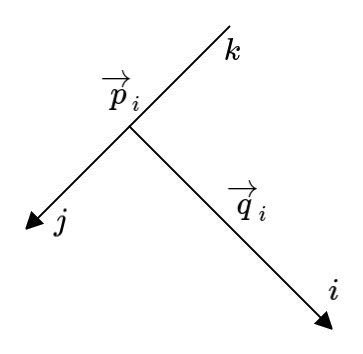
\includegraphics[width=0.3\textwidth,clip=true]{PhD-text/4_Formalism/jacobi_momenta_1.png}} 
\caption{Jacobi momenta $\vec{p}_{i}$ and $\vec{q}_{i}$ depending on suitable permutations.}
\label{fig:jacobi}
\end{figure}

The full 3N Hamiltonian reads 
\begin{equation}
H = H_{0} + V_{23} + V_{13} + V_{12} + V_{123}\;,
\end{equation}
where $H_{0} = \frac{\!\vec{\,p}^{2}}{m} + \frac{3}{4}\frac{\!\vec{\,q}^{2}}{m}$ is the free 3N Hamiltonian in the c.m. frame in terms of the Jacobi momenta, $V_{ij}$ denotes the NN potential acting between nucleons $i$ and $j$, and $V_{123}$ is the 3N potential, which can be always splitted to potential $V^{(i)}$ symmetric under the exchange of nucleons $j$ and $k$:
\begin{equation}
V_{123} = V^{(1)}_{4} + V^{(2)}_{4} + V^{(3)}_{4}\;,
\end{equation}
where $V^{(1)}_{4}$ is symmetric under the exchange of nucleons 2 and 3. In the case of three identical particles the totally antisymmetric state $\ket{\Psi}$ of three nucleons is given by
\begin{equation}
\begin{split}
\ket{\Psi} &= \ket{\psi_{1}} + \ket{\psi_{2}} + \ket{\psi_{3}} = (1+P)\ket{\psi_{1}}\;,
\end{split}
\end{equation}
where the permutation operator $P \equiv P_{12} P_{23} + P_{13} P_{23}$ is built from transmutations $P_{ij}$, which exchange particles $i$ and $j$ and $\ket{\psi_{1}}$ the Faddeev component of $\ket{\Psi}$. For example, the three-nucleon bound state $\ket{\Psi_{b}}$ fulfills the eigenvalue equation~\cite{nogga1997triton}
\begin{equation}
\ket{\psi_{1}} = G_{0} t P \ket{\psi_{1}}\;,
\end{equation}
where the two-nucleon $t$-operator obtaining by Eq.~(\ref{eqt}) acts now in the 3N space and $G_{0}$ is the free 3N propagator. For the 3N bound states, the energy argument of $G_{0}$ plays the role of the binding energy. 

The transition amplitude $U$ for the elastic Nd scattering is calculated prior to computing 3N scattering observables. Its matrix elements between the initial Nd $\ket{\phi}$ and final Nd $\ket{\phi^{\prime}}$ scattering state are given by~\cite{Glockle1996}
\begin{equation}
\begin{split}
\left<\phi^{\prime}|U|\phi\right> = \left<\phi^{\prime}|PG^{-1}_{0}|\phi\right> + \left<\phi^{\prime}|PT|\phi\right>\;.
\end{split}
\label{FaddeevElastic}
\end{equation}
For the deuteron breakup reaction the transition amplitude $U_{0}$ fulfils
\begin{equation}
\begin{split}
\left<\phi^{\prime}_{0}|U_{0}|\phi_{0}\right> = \left<\phi^{\prime}_{0}|(1 + P)T|\phi_{0}\right>\;,
\end{split}
\label{FaddeevBreakup}
\end{equation}
where $\ket{\phi^{\prime}_{0}}$ carries the information about the final free three-nucleon breakup channel.

The Faddeev equation for the auxiliary state $T\ket{\phi}$ for which nucleons interact via a NN interaction $V$ entering a $t$-matrix and a 3NF $V_{4}$ expressed as
\begin{equation}
\begin{split}
T\ket{\phi} &= t P \ket{\phi} + tP G_{0}T\ket{\phi} + (1 + tG_{0})V^{(1)}_{4}(1 + P)\ket{\phi} \\
&+(1 + tG_{0})V^{(1)}_{4}(1 + P)T\ket{\phi}\;,
\label{Faddeev1}
\end{split}
\end{equation}
where the initial state $\ket{\phi} = \ket{\varphi_{d}m_{d}}\ket{\vec{q}_{0}m_{N}}$ is composed of the deuteron wave function $\ket{\varphi_{d}}$ and a relative momentum eigenstate of the projectile nucleon, $\ket{\vec{q}_{0}}$, with corresponding the spin quantum numbers $m_{d}$ and $m_{N}$, respectively. 
%Further, $V^{(1)}_{4}$ is that part of $V_{4}$, which is symmetrical under the exchange of nucleons 2 and 3. 
This equation is the key equation for the nucleon-deuteron scattering and also the basis of predictions shown in this thesis. Neglecting the 3NF, Eq. (\ref{Faddeev1}) reduces to
\begin{equation}
\begin{split}
T\ket{\phi} &= t P \ket{\phi} + tP G_{0}T\ket{\phi}\;.
\label{Faddeev2}
\end{split}
\end{equation}

Now one can introduce momentum basis states for the 3N systems. 
We perform PWD of three-nucleons operators in $\ket{pq\alpha}$ basis
\begin{equation}
\begin{split}
&\ket{p q \alpha} \equiv \ket{pq \left(ls\right)j\left(\lambda\frac{1}{2}\right)I\left(j I\right)JM_{J}} \ket{\left(t\frac{1}{2}\right)TM_{T}}= \\
&\sum\limits_{m_{j}}C(jIJ;m_{j}, M_{J} - m_{j})\ket{p(ls)JM_{J}}\ket{q\left(\lambda\frac{1}{2}\right)I M_{J} - m_{j}}\\
&\sum\limits_{m_{t}}C(t\frac{1}{2}T;m_{t},M_{T} - m_{t})\ket{tm_{t}}\ket{\frac{1}{2}M_{T} - m_{t}}\;.
\end{split}
\label{pqalpha}
\end{equation}
Here, $l$, $s$, $j$, and $t$ denotes the orbital angular momentum, total spin, total angular momentum, and total isospin of the 2-3 c.m.s. subsystem, respectively, with $p = |\!\vec{\,p}|$ and $q = |\!\vec{\, q}|$ being the magnitudes of the Jacobi momenta $\vec{p}$.
% and $\vec{q}$, and with 2N spin states $\ket{sm_{s}}$ where $s$ = 0, 1. 
Next, the motion of nucleon 1 with respect to 2-3 c.m.s. subsystem is given in terms of the orbital momentum, $\lambda$ is coupled with its spin $\frac{1}{2}$ to give the total angular momentum of nucleon 1, $I$. Further, $j$ is coupled with $I$ to give the total angular momentum of the 3N system, $J$, with its projection $M_{J}$ on the quantization axis $\hat{z}$. Finally, $T$ and $M_{T}$ are the total 3N isospin and its projection. $T$ arises from coupling of 2N isospin $t$ = 0, 1 and the isospin $\frac{1}{2}$ of the nucleon 1. The $\ket{pq\alpha}$ basis is orthonormalized as
\begin{equation}
\begin{split}
\left<p^{\prime}q^{\prime}\alpha^{\prime}|pq\alpha\right> = \frac{\delta (q^{\prime} - q)}{qq^{\prime}}\frac{\delta (p^{\prime} - p)}{pp^{\prime}}\delta_{\alpha\alpha^{\prime}}\;,
%\delta^{(3)}\left(\!\vec{\,p}^{\prime} - \!\vec{\,p}\right)\delta^{(3)}\left(\!\vec{\,q}^{\prime} - \!\vec{\,q}\right)
\end{split}
\end{equation}
satisfies conditions of antisymmetrization of 2-3 subsystem by constraint $(-1)^{l+s+t} = -1$ and its normalization is
\begin{equation}
\sum\limits_{\alpha}\int\limits_{0}^{\infty}dp p^{2}\int\limits_{0}^{\infty}dq q^{2}\ket{pq\alpha}\bra{pq\alpha} = \mathds{1}\;.
%\int\mathrm{d}\vec{p}\mathrm{d}\vec{q}\ket{\!\vec{\,p}\!\vec{\,q}}\bra{\!\vec{\,p}\!\vec{\,q}} = \mathds{1}\;.
\end{equation}
%Tree nucleons are treated in spin-isospin formalism. Thus the 3N partial waves are built for a given $\vec{\mathcal{P}}$ from the subsystem 2-3 partial waves. Using the standard PWD with the set of discrete quantum numbers for the 3N system in the $j I$ coupling one can get $\ket{p q \alpha}$ states~\cite{Glockle1996}
%%
%The 3N system in partial-wave representation of Eq. (\ref{pqalpha}) requires the set of discrete quantum numbers $\alpha$ was chosen in a such way that $J = \frac{1}{2}$, $T = \frac{1}{2}$ with positive parity $(-1)^{l+\lambda} = 1$. To distinguish between $^{3}$H and $^{3}$He one has to be used $m_{T} = \frac{1}{2}$ and $m_{T} = -\frac{1}{2}$, correspondingly. 

%Now, I would like to outline the main keys , which well described in Refs.\cite{Glockle1996, glockle1983quantum}, but I will follow the description from Ref.~\cite{Glockle1996}. 
The first step of our way of the Faddeev equation~(\ref{Faddeev2}) is projection on the basis states of Eq.~(\ref{pqalpha})~\cite{Glockle1996, glockle1983quantum}
\begin{equation}
\begin{split}
\left<pq\alpha|T|\phi\right>  = &\left<pq\alpha|tP|\phi\right> + \sum\limits_{\alpha^{\prime}}\int\limits_{0}^{\infty}dp^{\prime}p^{\prime 2}\int\limits_{0}^{\infty}dq^{\prime}q^{\prime 2}\sum\limits_{\alpha^{\prime\prime}}\int\limits_{0}^{\infty}dp^{\prime\prime}p^{\prime\prime 2}\int\limits_{0}^{\infty}dq^{\prime\prime}q^{\prime\prime 2}\\
&\left<pq\alpha|t|p^{\prime} q^{\prime}\alpha^{\prime}\right>\left<p^{\prime}q^{\prime}\alpha^{\prime}|P|p^{\prime \prime} q^{\prime \prime}\alpha^{\prime \prime}\right>\left<p^{\prime\prime}q^{\prime\prime}\alpha^{\prime\prime}|G_{0}T|\phi\right>\;.
\end{split}
\label{firststep}
\end{equation}
The $t$-matrix is diagonal in the quantum numbers of the nucleon 1 
% It reads
\begin{equation}
\begin{split}
\left<pq\alpha|t(E)|p^{\prime} q^{\prime}\alpha^{\prime}\right> = &\frac{\delta (q - q^{\prime})}{qq^{\prime}}\delta_{\lambda\lambda^{\prime}}\delta_{ss^{\prime}}\delta_{tt^{\prime}}\delta_{jj^{\prime}}\delta_{II^{\prime}}\delta_{JJ^{\prime}}\delta_{m_{J}m_{J^{\prime}}}\delta_{TT^{\prime}}\delta_{m_{T}m_{T^{\prime}}} \\ &\tilde{t}_{\tilde{\alpha_{2}}\tilde{\alpha}^{\prime}_{2}}\left(p,p^{\prime}, E-\frac{3}{4}\frac{\!\vec{\,q}^{2}}{m}\right)\;,
\end{split}
\label{pqat2}
\end{equation}
where $\tilde{t}$ denotes the NN $t$-matrix and $\tilde{\alpha}_{2}$ contains the information about $lsjt$ components.
%with $\nu$ = -1, 0, 1 correspond to the $nn$, $np$ and $pp$ systems, respectively,

Assuming that $T = T^{\prime} = 1/2$, the two-nucleon $t$-matrix in the two-nucleon subsystem takes the form~\cite{witaa1989nucleon,witala2016role}
\begin{equation}
\left<\left(t\frac{1}{2}\right)T|t|\left(t^{\prime}\frac{1}{2}\right)T^{\prime}\right> = \delta_{tt^{\prime}}\delta_{TT^{\prime}}\delta_{T 1/2}\left[\delta_{t0}t^{t=0}_{np} + \delta_{t1}\left(\frac{2}{3}t^{t=1}_{nn} + \frac{1}{3}t^{t=1}_{np}\right)\right]\;.
\end{equation}
%In principle my investigations on elastic $nd$ scattering based on the idea from Ref.~\cite{witala2016role} which is for the elastic $nd$ scattering initial $T$ = $\frac{1}{2}$ state has dominant contributions of partial waves in case of using NN effective potential for obtaining the $t_{\mathrm{eff}}$-matrix as $t_{\mathrm{eff}} = \frac{2}{3}\tilde{t}_{nn} + \frac{1}{3}\tilde{t}_{np}$ with $t$=1 isospin states. 
For the elastic scattering the isospin $T = \frac{3}{2}$ components are negligible.
%, but they are becoming crucial in the calculation of the breakup reaction, see Section 6 of Ref.~\cite{Glockle1996} and results of Ref.~\cite{witala2016role}. However, the inclusion of $T = \frac{3}{2}$ partial-wave state it can be restricted to the 2N state $^{1}S_0$, which is characterized by the charge-independence breaking ($\tilde{t}_{nn} \neq \tilde{t}_{np}$), see Ref.~\cite{witala2016role}. 

%The computing of the matrix elements of the permutation operator for Eq.~(\ref{pqat2}) is one of the non-trivial problems in the 3-body problem. As was shown in Ref.~\cite{Glockle1996}, its the most common form reads as
Among various expressions for $\left< p^{\prime}q^{\prime}a^{\alpha}|P|pq\alpha \right>$ we use~\cite{Glockle1996}
\begin{equation}
\begin{split}
&\left<p^{\prime} q^{\prime}\alpha^{\prime}|P|pq\alpha\right> = \int\limits_{-1}^{1}dx\frac{\delta (p^{\prime} - \pi_{1})}{p^{\prime l^{\prime} + 2}}\frac{\delta (p - \pi_{2})}{p^{\prime l + 2}}G_{\alpha^{\prime}\alpha}(q^{\prime}q x)\;,
\end{split}
\label{permutation1}
\end{equation}
where 
\begin{equation}
\pi_{1} = \sqrt{q^{2} + \frac{1}{4}q^{\prime 2} qq^{\prime}x}\;,~\pi_{2} = \sqrt{q^{\prime 2} + \frac{1}{4}q^{\prime 2} qq^{\prime}x}\;,
\end{equation}
and $G_{\alpha^{\prime}\alpha}(q^{\prime}q x)$ is a purely geometrical quantity.

The three-nucleon propagator in partial-wave basis is
\begin{equation}
\left<pq\alpha|G_{0}|p^{\prime}q^{\prime}\alpha^{\prime}\right> = \frac{1}{E - \frac{p^{2}}{m} - \frac{3}{4m}q^{2}}\frac{\delta (q - q^{\prime})}{qq^{\prime}}\frac{\delta (p - p^{\prime})}{pp^{\prime}}\delta_{\alpha\alpha^{\prime}}\;.
\end{equation}

Inserting decompositions~(\ref{firststep}) and~(\ref{pqat2}) and reducing  momenta integrations with help of $\delta$-functions one gets
\begin{equation}
\begin{split}
\left<pq\alpha|T|\phi\right> &= \sum\limits_{\alpha^{\prime}}\int\limits_{-1}^{1}dx\frac{\tilde{t}_{\tilde{\alpha}\tilde{\alpha}^{\prime}}(p,\pi_{1},E-(3/4)q^{2})}{\pi^{l^{\prime}}_{1}}\sum\limits_{\alpha^{\prime\prime}}\delta_{\alpha^{\prime\prime}\alpha_{d}}G_{\alpha^{\prime}\alpha^{\prime\prime}}(q,q_{0},x)\frac{\varphi_{l^{\prime\prime}}(\pi_{2})}{\pi^{l^{\prime\prime}}_{2}}C^{m_{d}m_{N}}_{\alpha^{\prime\prime}} \\&+ \sum\limits_{\alpha^{\prime}}\sum\limits_{\alpha^{\prime\prime}}\int\limits_{0}^{\infty}dq^{\prime}q^{\prime 2}\int\limits_{-1}^{1}dx\frac{\tilde{t}_{\tilde{\alpha}\tilde{\alpha}^{\prime}}(p,\pi_{1},E-(3/4)q^{2})}{\pi^{l^{\prime}}_{1}}\\
&\times G_{\alpha^{\prime}\alpha^{\prime\prime}}(qq^{\prime}x)\frac{1}{E + i\varepsilon - q^{2}/m - q^{\prime 2}/m - qq^{\prime}x/m}\frac{\left<\pi_{2}q^{\prime}\alpha^{\prime\prime}|T|\phi\right>}{\pi^{l^{\prime\prime}}_{2}}\;,
\end{split}
\label{eqF1}
\end{equation}
%with
%\begin{equation}
%\begin{split}
%\left<pq\alpha|tP|\phi\right> &= \sum\limits_{\alpha^{\prime}}\int\limits_{-1}^{1}dx\frac{\tilde{t}_{\tilde{\alpha}\tilde{\alpha}^{\prime}}(p,\pi_{1},E-(3/4)q^{2})}{\pi^{l^{\prime}}_{1}}\\&\sum\limits_{\alpha^{\prime\prime}}\delta_{\alpha^{\prime\prime}\alpha_{d}}G_{\alpha^{\prime}\alpha^{\prime\prime}}(q,q_{0},x)\frac{\varphi_{l^{\prime\prime}}(\pi_{2})}{\pi^{l^{\prime\prime}}_{2}}C^{m_{d}m_{N}}_{\alpha^{\prime\prime}}\;,
%\label{eqF11}
%\end{split}
%\end{equation}
where
\begin{equation}
\begin{split}
C^{m_{d}m_{N}}_{\alpha^{\prime\prime}} = \sqrt{\frac{2\lambda + 1}{4\pi}}C\left(\lambda\frac{1}{2}I,0m_{N}\right)C\left(1IJ,m_{d}m_{N}\right)\;,
\label{eqF12}
\end{split}
\end{equation}
and $\alpha_{d}$ denotes the set of discrete quantum numbers for the 2N subsystem containing the deuteron quantum numbers $l = 0, 2$, $s = 1$, $j = 1$, and $t = 0$.

In all my numerical 3N calculations, Eq.~(\ref{Faddeev2}) is solved numerically by generating its Neumann series which
is next summed up using the Pad\`e method~\cite{Glockle1996, glockle1983quantum}. The partial wave basis comprising 3N states includes all states with the two-body subsystem total angular momentum $j$ $\leq$ 5 and the total 3N angular momentum $J$ $\leq$ $\frac{25}{2}$. This guarantes convergence of predictions with respect to the total angular momenta. The total number of three-nucleon channels states $\ket{\alpha}$ for gieven $J$ amounts up to 142. The range and size of grid points representing momenta $p$ and $q$ are chosen adjusted separately for each of the potential models. I use grids of 32 $p$ points in the range 0-40 $\mathrm{fm}^{-1}$ and 37 $q$ points in the range 0-25 $\mathrm{fm}^{-1}$ in case of for the chiral SMS force and the OPE-Gaussian potential.  
%For investigation presented here we use all
%what is sufficient to guarantee convergence of our
%partial waves with j max ≤ 5 and J ≤ 25
%2
%predictions at the energies discussed in this paper
%
%It will be solved numerically, in the basis |p, q, α>, by generating its Neumann series which is next summed up using the Pade method [32,33]. All two-body states with the total angular momentum $j \leq 5$ and all three-body states with the total angular momentum $J \leq 25/2$ will be taken into account. This guarantes convergence of our predictions with respect to the number of partial waves and thus also sufficient accuracy of planned calculations will be achieved. The total number of three-nucleon channels in the basis |α> will amount up to 142, when solving the equation for T|Φ> separately for each total angular momentum and parity of the 3N system.

\subsection{3N scattering observables}
The 3N scattering processes are characterized by a large set of spin-observables. In addition to the polarized differential cross section and the vector analyzing powers of nucleons, there are also vector and tensor analyzing powers of the deuteron. Further
information on the dynamics can be found from the spin transfer and the spin-correlation coefficients. In total, there are 55 different observables for the elastic scattering.
By solving Eqs. (\ref{eqF1}) and~(\ref{FaddeevElastic}) one find the elastic transition amplitude $U$. It is directly related to the physical elastic scattering amplitude taking into account various polarization states
\begin{equation}
M_{ij} \equiv -\frac{2}{3}m(2\pi)^{2}\left<\phi^{\prime}|U|\phi\right> = -\frac{2}{3}m(2\pi)^{2}\left<\phi^{\prime}_{j}|U|\phi_{i}\right>\;,
\end{equation}
where $i,j$ denote denote the initial and final spin states, respectively. From $M_{ij}$ any elastic 3N observable can be computed.

For example, the polarized differential cross section for the elastic Nd scattering in the c.m.s. equals
\begin{equation}
\frac{d\sigma}{d\Omega} = |M_{m^{\prime}_{d}m^{\prime}_{N}m_{d}m_{N}}(\!\vec{\,q}^{\prime},\vec{q}_{0})|^{2}\;,
\end{equation}
%with
%\begin{equation}
%M_{m^{\prime}_{d}m^{\prime}_{N}m_{d}m_{N}}(\!\vec{\,q}^{\prime},\vec{q}_{0}) = -\frac{2}{3}m(2\pi)^{2}\left<\phi^{\prime}|U|\phi\right>\;,
%\end{equation}
where $\vec{q}_{0}$ is the relative momentum of the incident nucleon with respect to the deuteron, and $\!\vec{\, q}^{\prime}$ describes the same momentum in the final state. More general representation for the spin-averaged (unpolarized) differential cross section is given by 
\begin{equation}
\frac{d\sigma}{d\Omega} \equiv I_{0} = \frac{1}{6}\mathrm{Tr}(MM^{\dagger})\;,
\end{equation}
with trace taken over spin states.

%With regard to the deuteron breakup process, after solving Eq. (\ref{eqF1}) we get both $T = 1/2(\left<pq\alpha|T|\phi\right>)$ and $T = 3/2(\left<pq\beta|T|\phi\right>)$ amplitudes from which the breakup $\left<\phi_{0}|U_{0}|\phi\right>$ amplitude can be found. The $\ket{pq\beta}$ and $\ket{pq\alpha}$ states are related
%\begin{equation}
%\ket{pq\beta} = \sum\limits_{j, I}\sqrt{\hat{j}\hat{I}\hat{L}\hat{S}}
%\left\lbrace\begin{matrix} l&s&j \\ \lambda &\frac{1}{2}&I\\L&I&J \end{matrix}\right\rbrace\ket{pq\alpha}\;,
%\end{equation}
%and vice verse
%\begin{equation}
%\ket{pq\alpha} = \sum\limits_{L,S}\sqrt{\hat{j}\hat{I}\hat{L}\hat{S}}
%\left\lbrace\begin{matrix} l&s&j \\ \lambda &\frac{1}{2}&I\\L&S&J \end{matrix}\right\rbrace\ket{pq\beta}\;,
%\end{equation}
%where $\lbrace\ldots\rbrace$ refers to the Wigner 9-j symbol~\cite{Weisstein} as an alternative to Clebsch–Gordan coefficients.
In case of the deuteron breakup, the five-fold differential cross section in the c.m.s. is given as
\begin{equation}
\frac{d^{5}\sigma}{d\hat{p}d\hat{q}dq} = \frac{(2\pi)^{4}m^{2}}{3q_{0}}pq^{2}|\left<\phi_{0}|U_{0}|\phi\right>|^{2}\;.
\end{equation}
In practice, depending on the kinematically allowed configuration, $\frac{d^{5}\sigma}{d\hat{p}d\hat{q}dq}$ can be expressed as a function of laboratory scattering angles, $\frac{d^{5}\sigma}{d\Omega_{1}d\Omega_{2}dE}$, and the arc-length of the S-curve,$\frac{d^{5}\sigma}{d\Omega_{1}d\Omega_{2}dS}$, see Ref.~\cite{Glockle1996}. In principle, this is also valid for to polarized various 3N breakup  polarization observables.

The same representation allows to define the spin observables~\cite{Glockle1996}. The initial state polarization of the nucleon leads to the definition of the nucleon analyzing powers
\begin{equation}
A_{k}(N) \equiv \frac{\mathrm{Tr}(M\sigma_{k}M^{\dagger})}{\mathrm{Tr}(MM^{\dagger})}\;.
\end{equation}
Using the common convention to choose the scattering plane as the $x-z$ plane and the $y$ axis pointing to the direction $\vec{k}_{in}\times\vec{k}_{out}$, where $\vec{k}_{in}$ and $\vec{k}_{out}$ are the momenta of the incoming and outgoing nucleons, respectively, results in non-zero the nucleon vector analyzing power $A_{y}(N)$, while $A_{x}(N) = A_{z}(N) = 0$.

The deuteron vector and the tensor polarizations of the deuteron in the initial state leads to the vector $A_{i}$ and the tensor $A_{jk}$ analyzing powers of the deuteron, respectively,
\begin{equation}
A_{i} = \frac{\mathrm{Tr}(M\mathcal{P}_{i}M^{\dagger})}{MM^{\dagger}}\;,~A_{jk} = \frac{\mathrm{Tr}(M\mathcal{P}_{jk}M^{\dagger})}{MM^{\dagger}}\;,
\end{equation}
where $\mathcal{P}_{i}$ is the polarization vector and $\mathcal{P}_{jk}$ is the polarization tensor. The parity conservation reduces the number of observables resulting in only vector and three tensor analyzing powers
\begin{equation}
iT_{11} = \frac{\sqrt{3}}{2}A_{y}\;,~T_{20} = \frac{1}{\sqrt{2}}A_{zz}\;,~T_{21} = -\frac{1}{\sqrt{3}}A_{xz}\;,~T_{22} = \frac{1}{2\sqrt{3}}(A_{xx} - A_{yy})\;.
\end{equation}

When, both the incident nucleon and the deuteron are polarized in the initial state various spin-correlation coefficients $C_{j,k}$ and $C_{jk, i}$ occures. In the case when one particle s polarized in the initial state and one in the final state we deal with the spin transfer coefficients $K^{l^{\prime}}_{k}$ and $K^{li^{\prime}}_{k}$. 
%Obviously, the number of such quantities can be reduced due to the parity conservation and the time-reversal symmetry. 

All those above-mentioned quantities depend on the scattering angle and reaction energy.
Extending the above definitions one can define the spin observables in the deuteron breakup process for which the number of 3N observables is much greater than for the elastic scattering.
%thus the Faddeev component $\kef.et{\psi_{b}}$ for the 3N bound state in PWD is written as
%\begin{equation}
%\begin{split}
%\braket{pq\alpha}{\psi_{b}} = \sum\limits_{\alpha^{\prime}}\int\limits_{0}^{\infty}dp^{\prime}p^{\prime 2}\int\limits_{0}^{\infty}dq^{\prime}q^{\prime 2}\Psi (p,q,\alpha^{\prime})\ket{pq\alpha^{\prime}}
%%\ket{pq\alpha^{\prime}}\bra{p^{\prime}q^{\prime}\alpha^{\prime}}
%\end{split}
%\end{equation}

%which
%belongs to standard techniques used to investigate 3N reactions. This approach is described in detail e.g. in~\cite{Witaa2001, Glockle1996, glockle1983quantum}.
%
%The formalism of the momentum space Faddeev equation
%is one of the standard techniques to investigate 3N reactions
%and has been described in detail many times; see, e.g., [44,45].
%Thus we only briefly remind the reader of its key elements.
%
%For a given N N interaction V we solve the Lippmann-
%Schwinger equation t = V + V G̃ 0 t to obtain matrix elements
%of the 2N t operator, with G̃ 0 being the 2N free propagator.
%These matrix elements enter the 3N Faddeev scattering equa-
%tion which, neglecting the 3N force, takes the following form:


%\chapter{Various types of theoretical uncertainties for the elastic Nd scattering observables}
%%Propagation of uncertainties of the NN\\ potentials}
%\label{error}
%The quantification of uncertainties in theoretical calculations for nuclear observables is a very up-to-date topic.  Due to increasing computing power, it has become possible to use statistical methods in theoretical low-energy nuclear physics that allows performing error propagation. So this thesis has an interdisciplinary character. In this Chapter, we describe various types of theoretical uncertainties presented in the studies on elastic and breakup Nd processes by performing calculations with the Faddeev equation.
%\section{Determination of statistical uncertainty in a 3N \\system}
%\label{statistical}
%We have repeatedly mentioned above the importance of the covariance matrix of NN potential parameters to use a statistical approach to estimate theoretical uncertainties, which we also call the statistical uncertainties. Drawing on our procedure of determining the theoretical uncertainty arising from the NN potential parameters, which was described in ~\cite{Skibinski2018}, the statistical uncertainty can be found by the following steps:
%\begin{enumerate}
%\item Preparation of sets of the potential parameters.
%
%The potential parameters for the chiral interaction result from $\chi^{2}$ fitting of theoretical predictions directly to the data collected in the Granada database~\cite{Perez2013}. The fitting procedure is described in detail in Refs.~\cite{Reinert2018} and~\cite{ReinertMaster}. As a result, the central values of the parameters and their covariance matrix are obtained. Being in contact with members of the Bochum-Bonn group we received the set ($S_{0}$) of expectation values and the covariance matrices of potential parameters for all orders of chiral expansion. The various sets of potential parameters have been computed by sampling from the multivariate normal distribution (in space of parameters) with a given covariance matrix. The multivariate sampling was done using the Mathematica\textsuperscript{\textregistered}~\cite{Mathematica11p3} computing system. As a result, we sampled 50 sets ($S_{i}, i = 1 \ldots 50)$ of NN potential parameters. Also in the case of the OPE-Gaussian interaction, we are already in contact with authors of this potential and have been equipped by them with the set of the central values of the parameters and a sample of 50 sets of potential parameters. Such a number of sets guarantee a statistically meaningful probe. Since the OPE-Gaussian force was derived in coordinate space, the additional transformation of its matrix elements from coordinate space to momentum space was done. This was achieved by the standard transformation formula which requires numerical integrations involving spherical Bessel functions. 
%\item Calculation of the deuteron properties: binding energy, $^{3}S_{1}$ and $^{3}D_{1}$ state probabilities.
%
%For each set $S_{i}~(i = 0,1, \ldots, 50)$ we calculated the deuteron wave-function by solving the Schr{\"o}dinger equation in momentum space. In this case Schr{\"o}dinger equation can be expressed as an eigenvalue problem. The solutions of this problem -- eigenvalue which corresponds to the binding energy and corresponding eigenvector which can be directly linked to the deuteron wave function -- were obtained using the standard numerical methods~\cite{numrecipesFortran} and the LAPACK library. Calculation of the deuteron was performed for all investigated models of interaction.
%
%\item Calculation of the NN scattering observables: unpolarized cross section and various polarization observables at a few various energies of the reaction up to 200~MeV.
%
%The computation of the NN scattering observables requires a calculation of the transition amplitude between initial and final two-nucleon states. The amplitude is given as the matrix element of the $t$-operator, which is a solution of the Lippmann-Schwinger equation. Thus during this step, we solved, again for each of the investigated models of interaction and all sets of parameter values, this equation and after the suitable anti-symmetrization, the transition amplitude and the observables were computed~\cite{glockle1983quantum, Glockle1996}.   
%
%\item Calculation of the nucleon-deuteron scattering observables.
%%
%%and the t matrix, solved, at
%%each considered energy, the Faddeev equation (2.1),
%%calculated the scattering amplitude [Eq. (2.2)], and
%%finally computed observables. As a result the angular
%%dependence of various scattering observables is known
%%for each set of parameters S i .
%\end{enumerate}
%\section{Description of truncation errors}
%\label{truncation}
%\section{Bayesian statistics for truncation errors}
%\label{bayes}
%%%%%%%%%%%%%%%%%%%%%%%%%%%%%%%%%%%%%%%%%%%%%%%%%%%%%
%\section{Statistical quantities used}
%\label{stat}


%%%%%%%%%%%%%%%%%%%%%%%%%%%%%%%%%%%%%%%%%%%%%%%%%%%%%
% Import the acknowledgments.                       %
%%%%%%%%%%%%%%%%%%%%%%%%%%%%%%%%%%%%%%%%%%%%%%%%%%%%%
%\input{PhD-text/Acknowledgments/acknowledgments.tex}

%%%%%%%%%%%%%%%%%%%%%%%%%%%%%%%%%%%%%%%%%%%%%%%%%%%%%
% This generates the bibliography.                  %
%%%%%%%%%%%%%%%%%%%%%%%%%%%%%%%%%%%%%%%%%%%%%%%%%%%%%
\bibliographystyle{unsrt}
\bibliography{mybib}
%\input{PhD-text/Bibliography/bibliography.tex}
%\input{PhD-text/Bibliography/library}

\end{document}
